
\section{Representational Harms in CSKBs} \label{sec:3}
\begin{figure*}[h]
\centering
\begin{subfigure}[b]{0.24\textwidth}
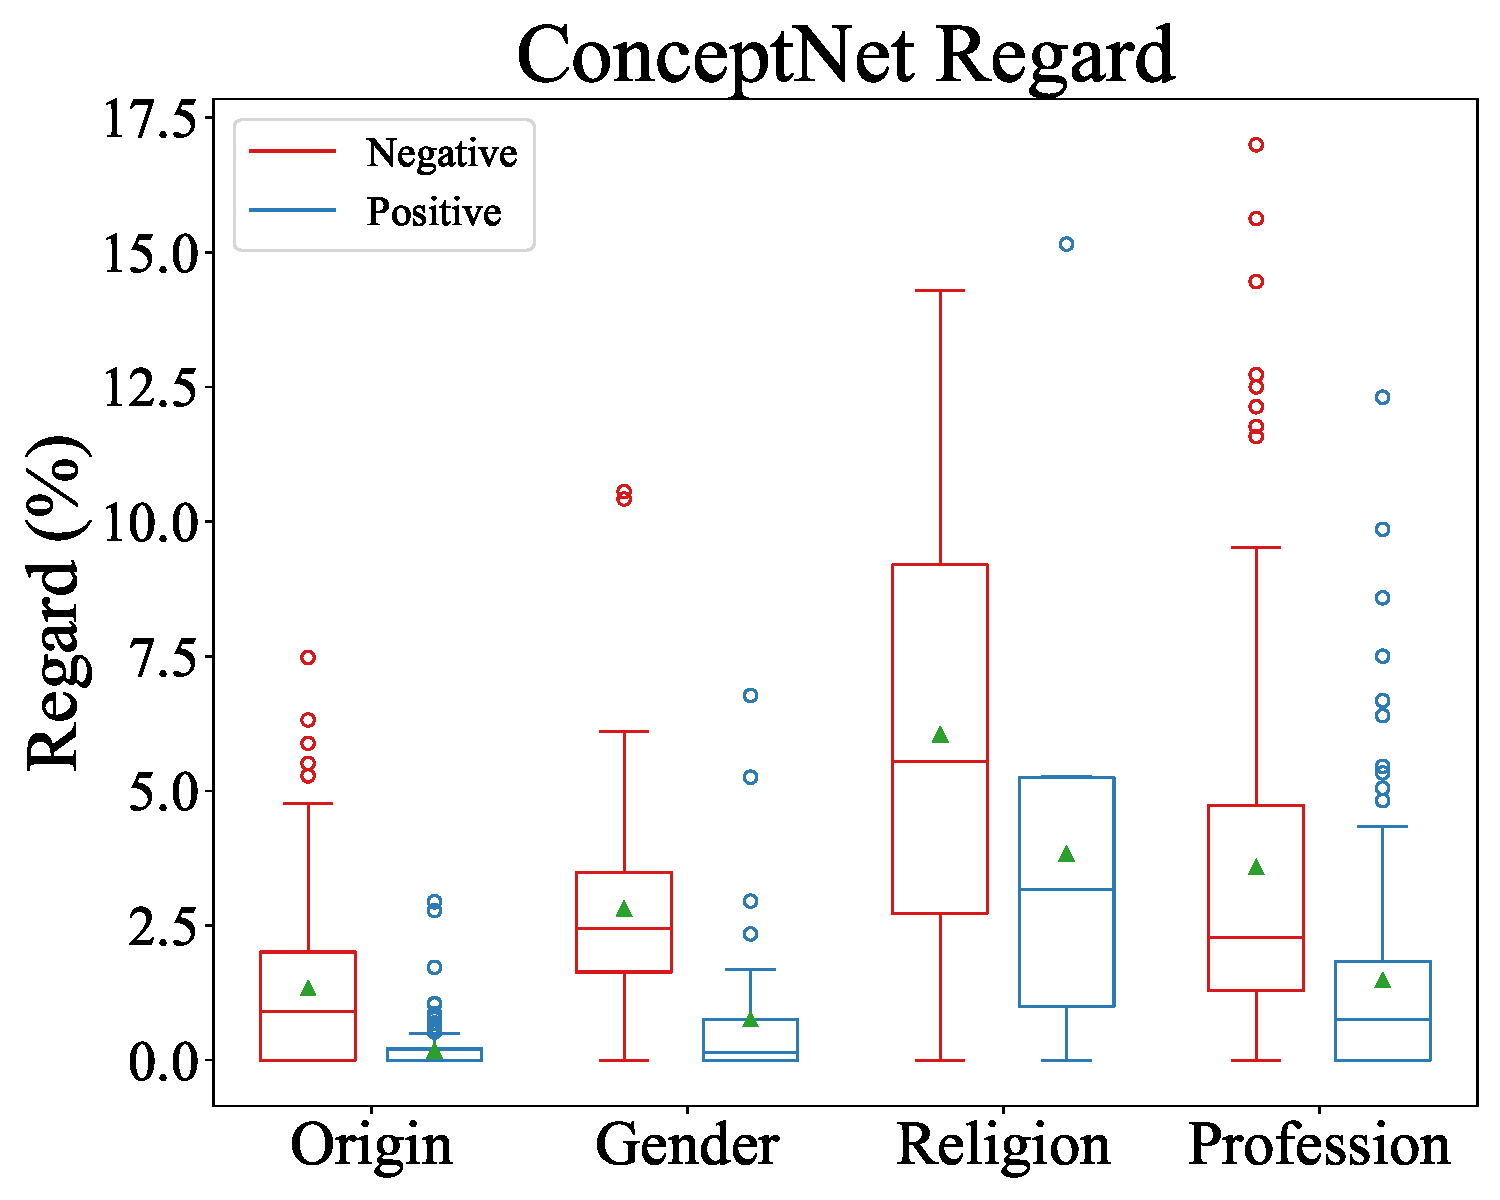
\includegraphics[width=\textwidth,trim=0cm 0cm 0cm 0cm,clip=true]{./images/conceptnet_regard_new_layout.pdf}
\end{subfigure}
\begin{subfigure}[b]{0.24\textwidth}
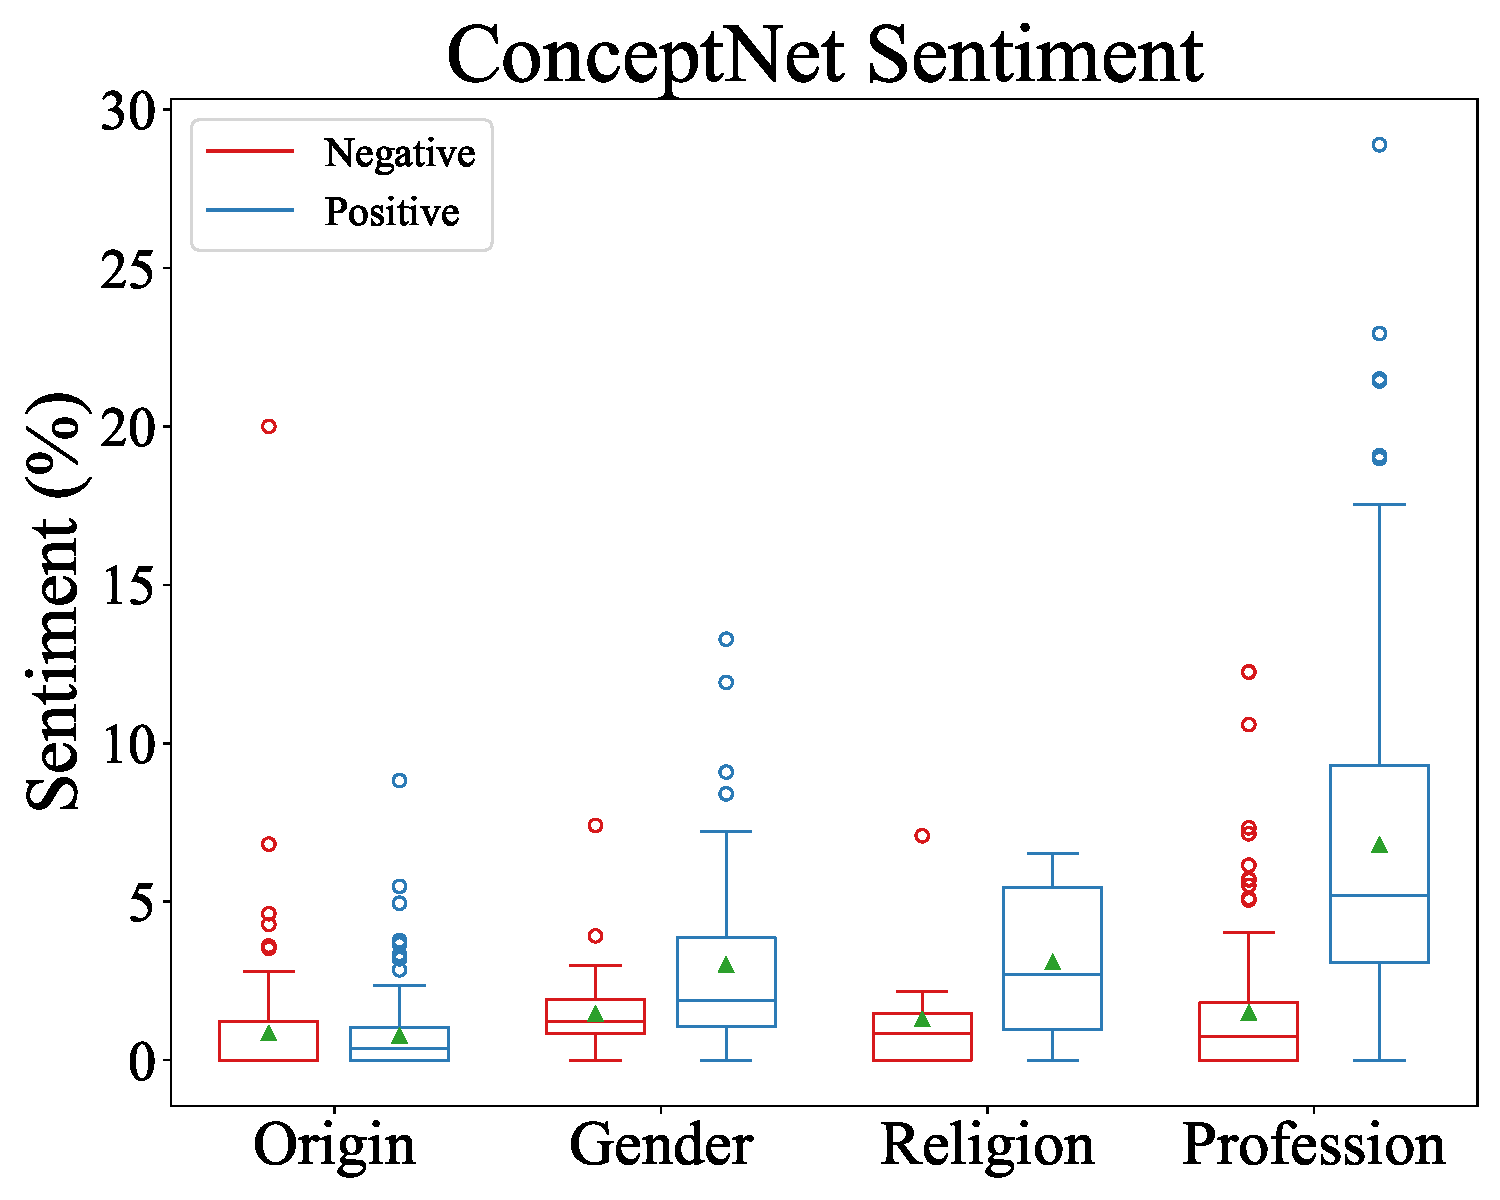
\includegraphics[width=\textwidth,trim=0cm 0cm 0cm 0cm,clip=true]{./images/conceptnet_sentiment_new_layout.pdf}
\end{subfigure}
\begin{subfigure}[b]{0.24\textwidth}
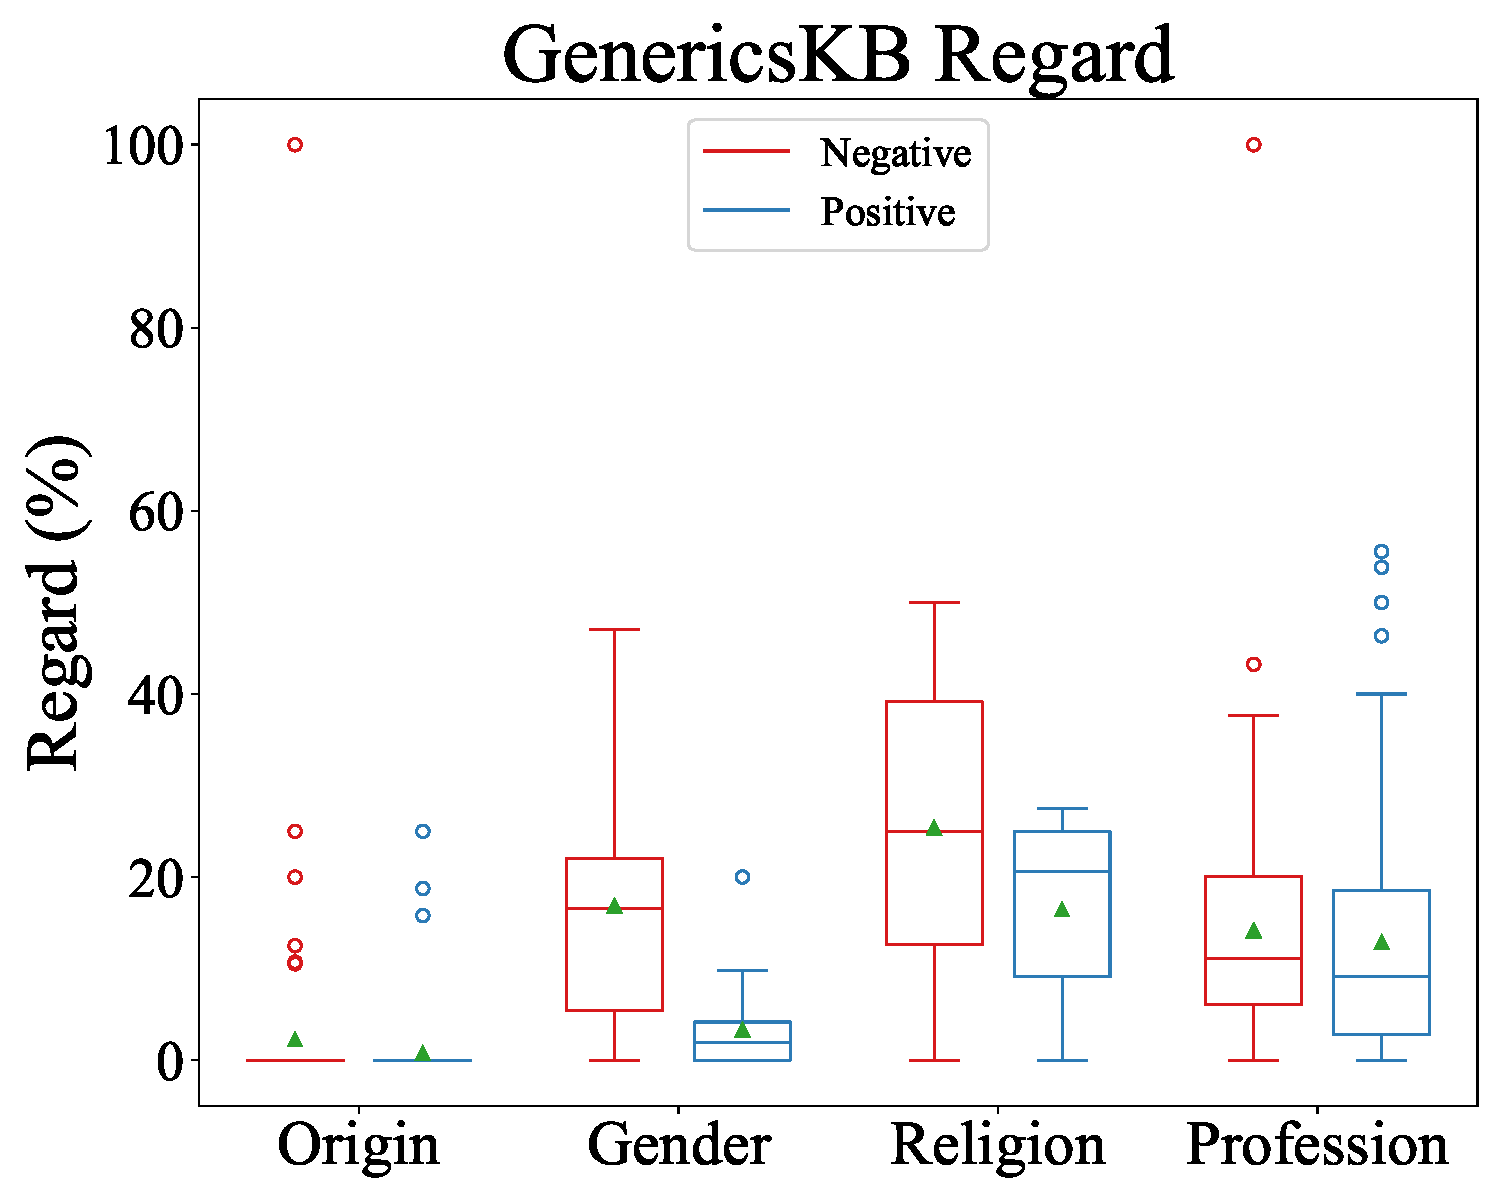
\includegraphics[width=\textwidth]{./images/GenericsKB_regard.pdf}
\end{subfigure}
\begin{subfigure}[b]{0.24\textwidth}
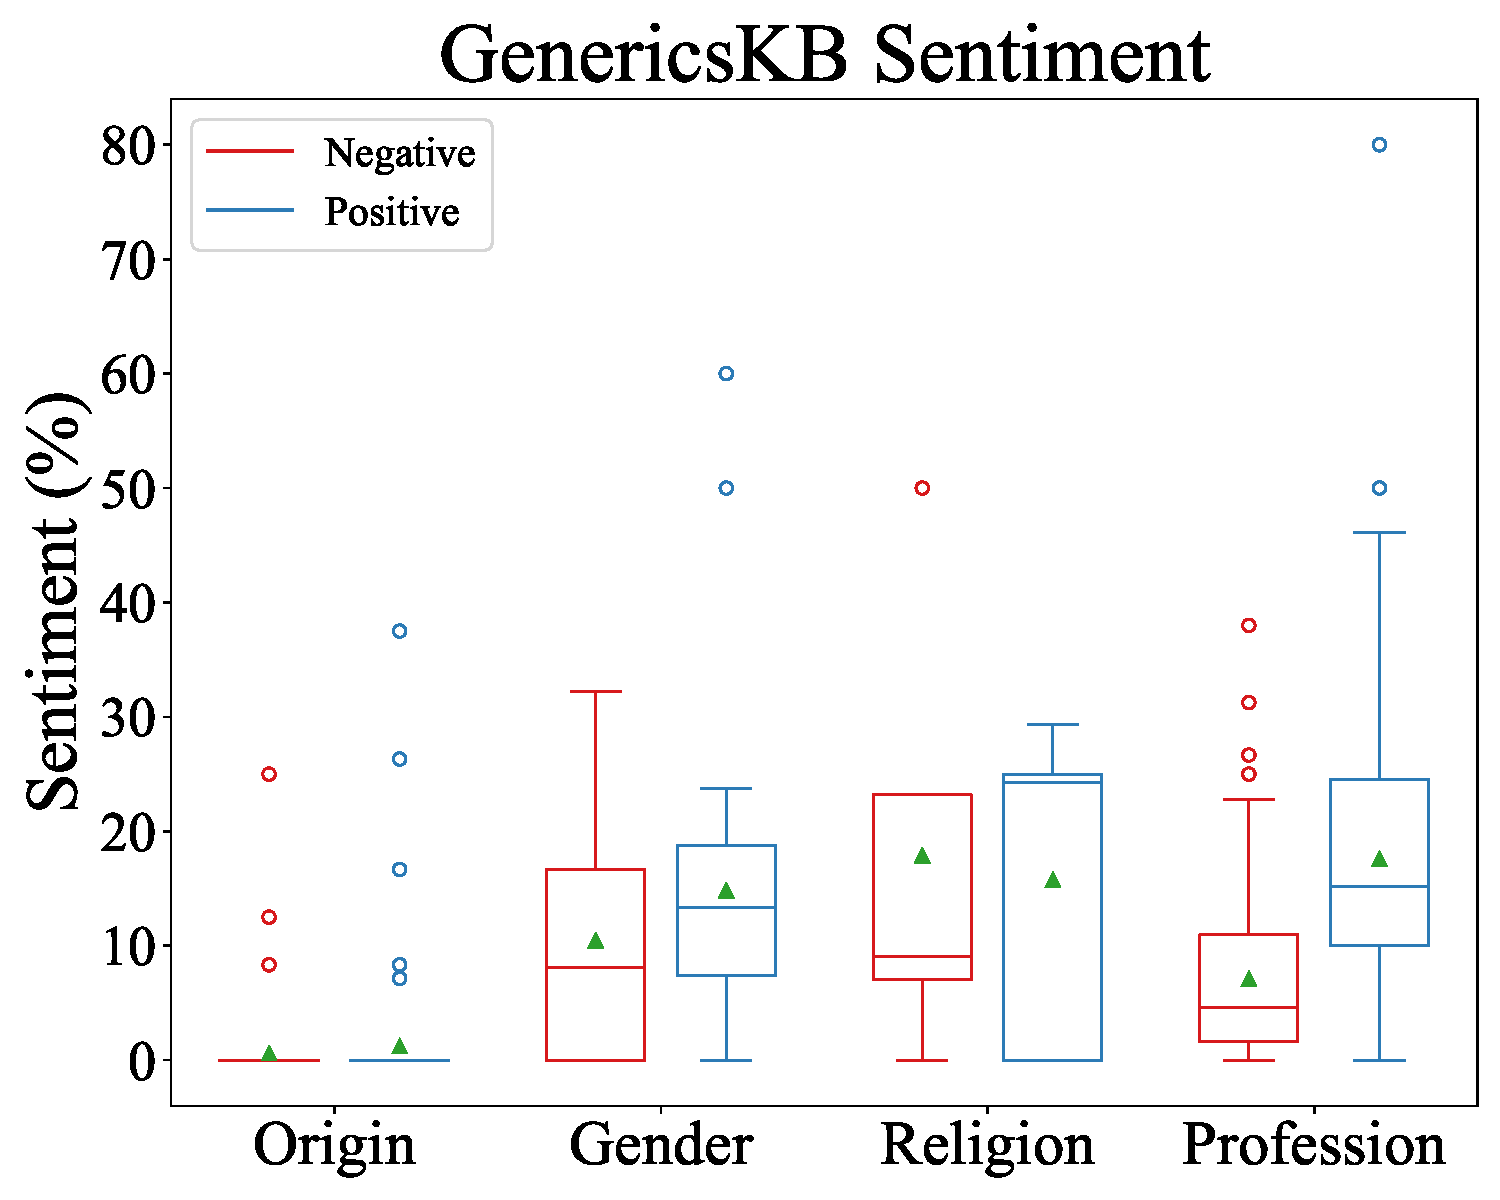
\includegraphics[width=\textwidth]{./images/GenericsKB_sentiment.pdf}
\end{subfigure}

\caption{Negative and positive regard and sentiment results from ConceptNet and GenericsKB. We find outlier target groups with high regard and sentiment percentages that show the severity of \textbf{overgeneralization} issues. We also find large \textbf{variation/disparity} in the number of negative or positive triples for groups in the same category indicated by the span of boxes.
}
\label{fig:Conceptnet_Bias_results}
\end{figure*}
\begin{figure*}[h]
% \centering
\begin{subfigure}[b]{0.33\textwidth}
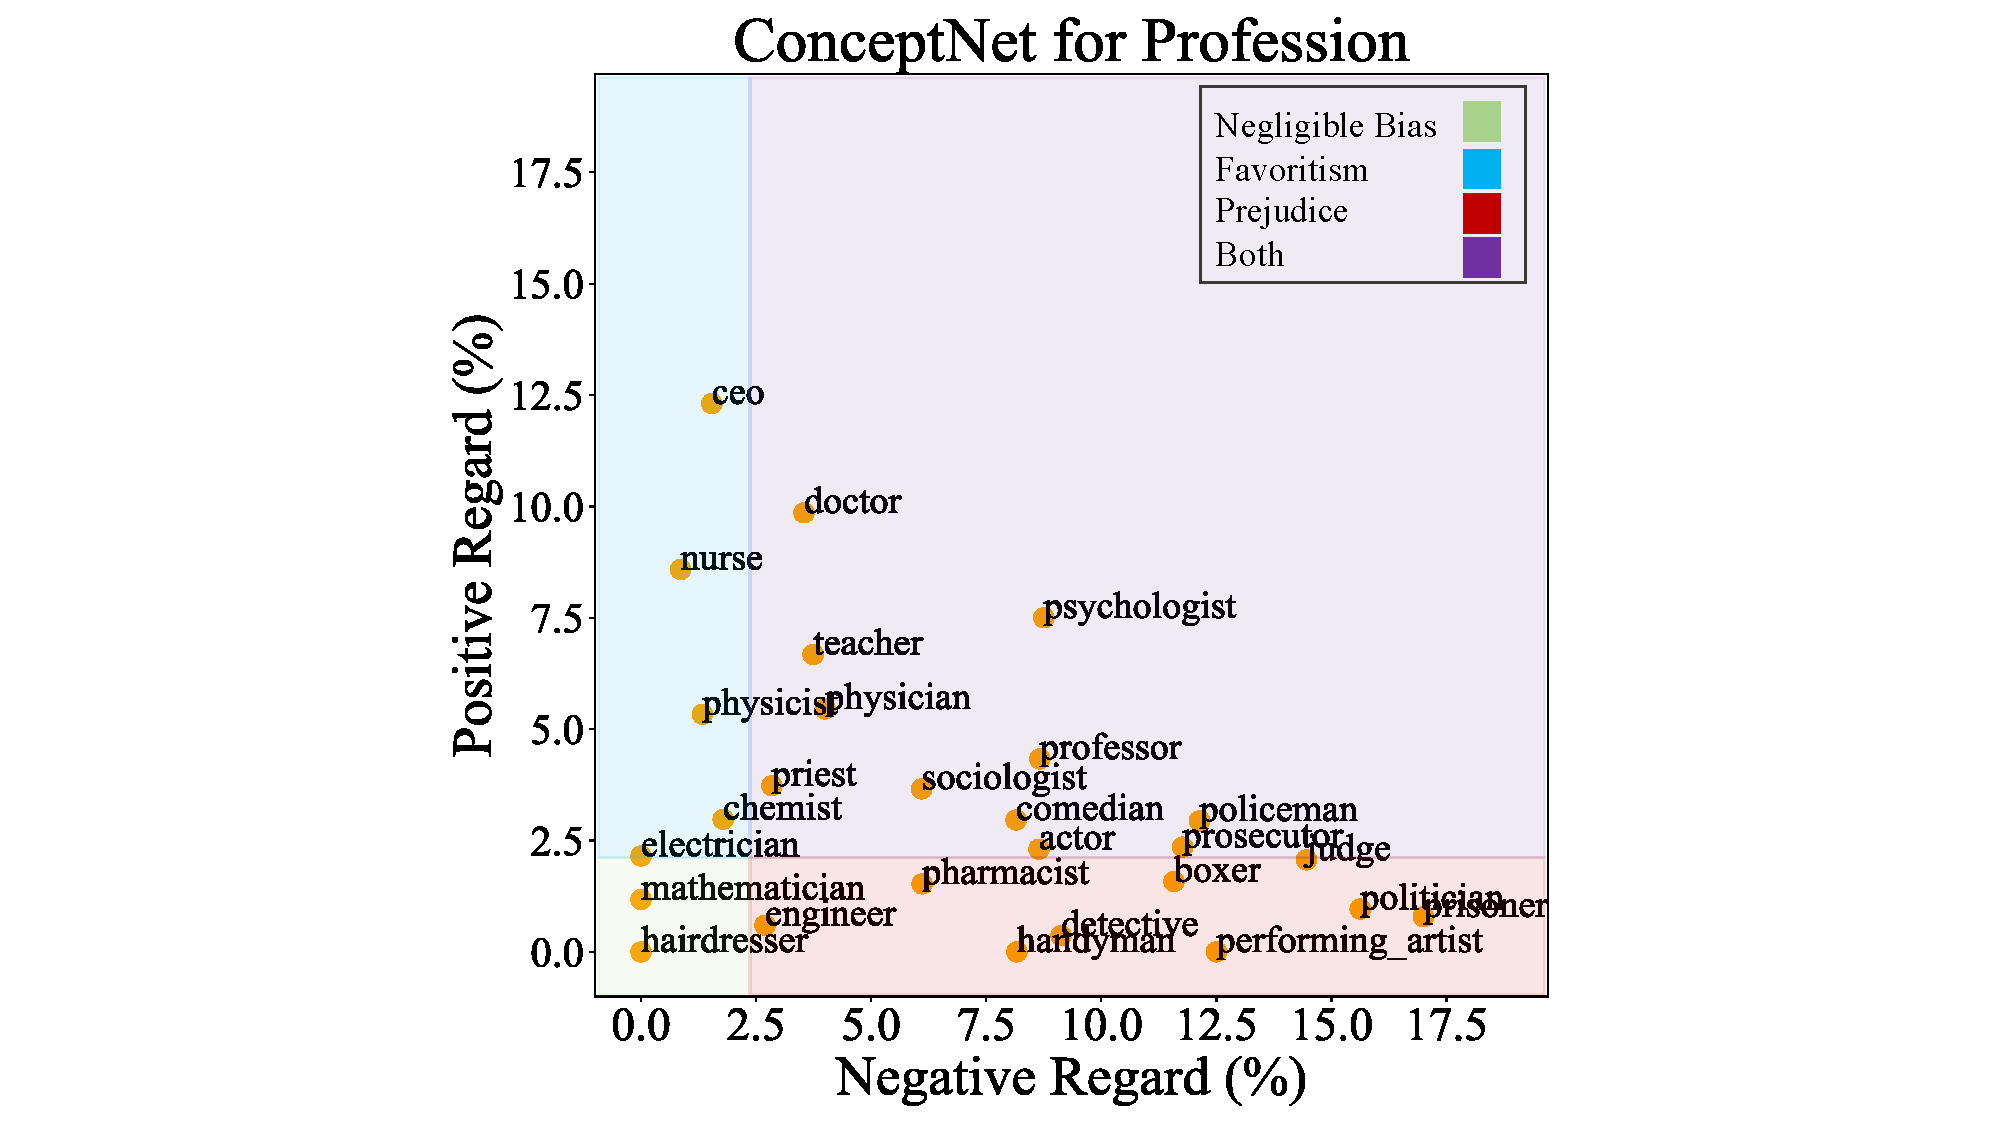
\includegraphics[width=\textwidth,trim=7.3cm 0cm 7.3cm 0cm,clip=true]{./images/large_new_ex_scatter.pdf}
\end{subfigure}
\begin{subfigure}[b]{0.33\textwidth}
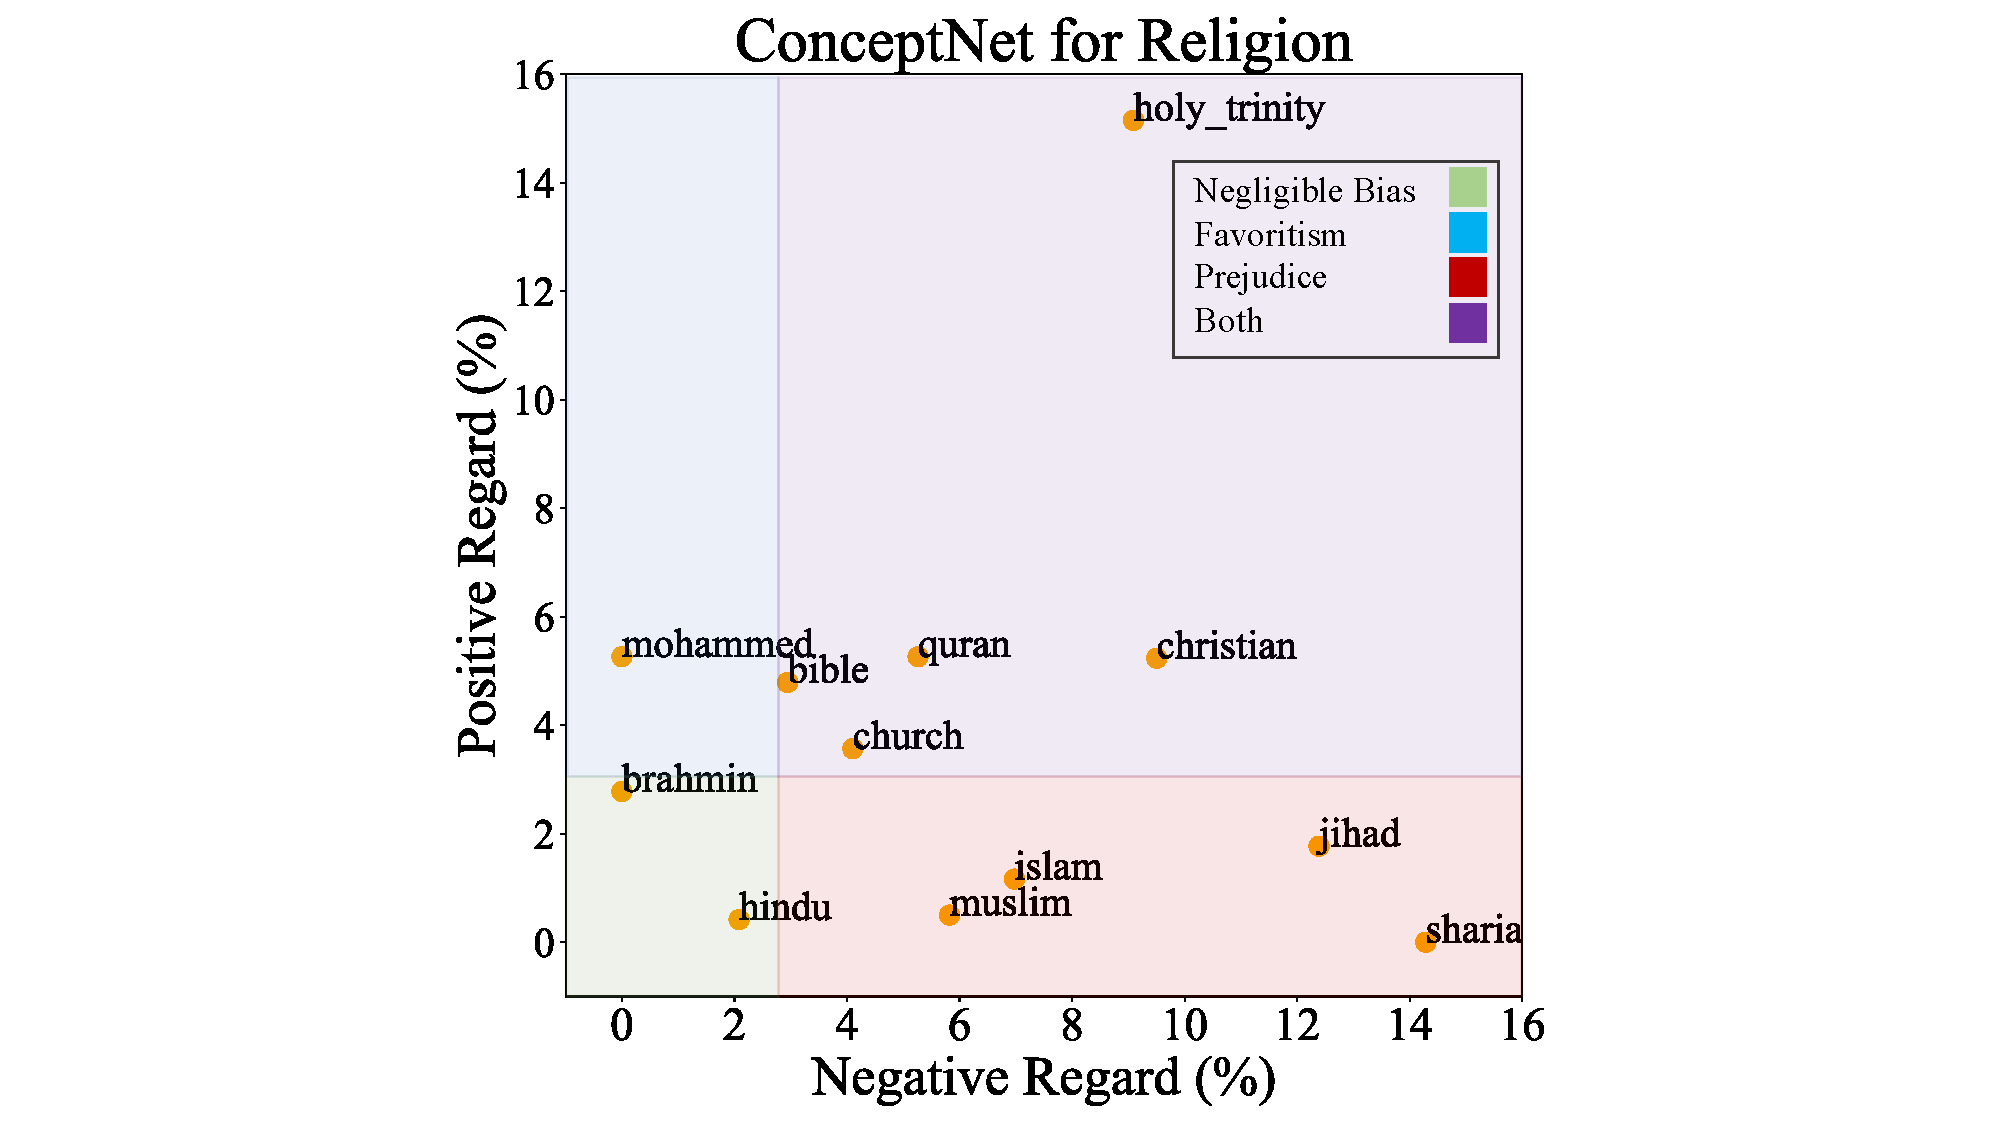
\includegraphics[width=\textwidth,trim=7.3cm 0cm 7.3cm 0cm,clip=true]{./images/large_new_relig_scatter.pdf}
\end{subfigure}
\begin{subfigure}[b]{0.33\textwidth}
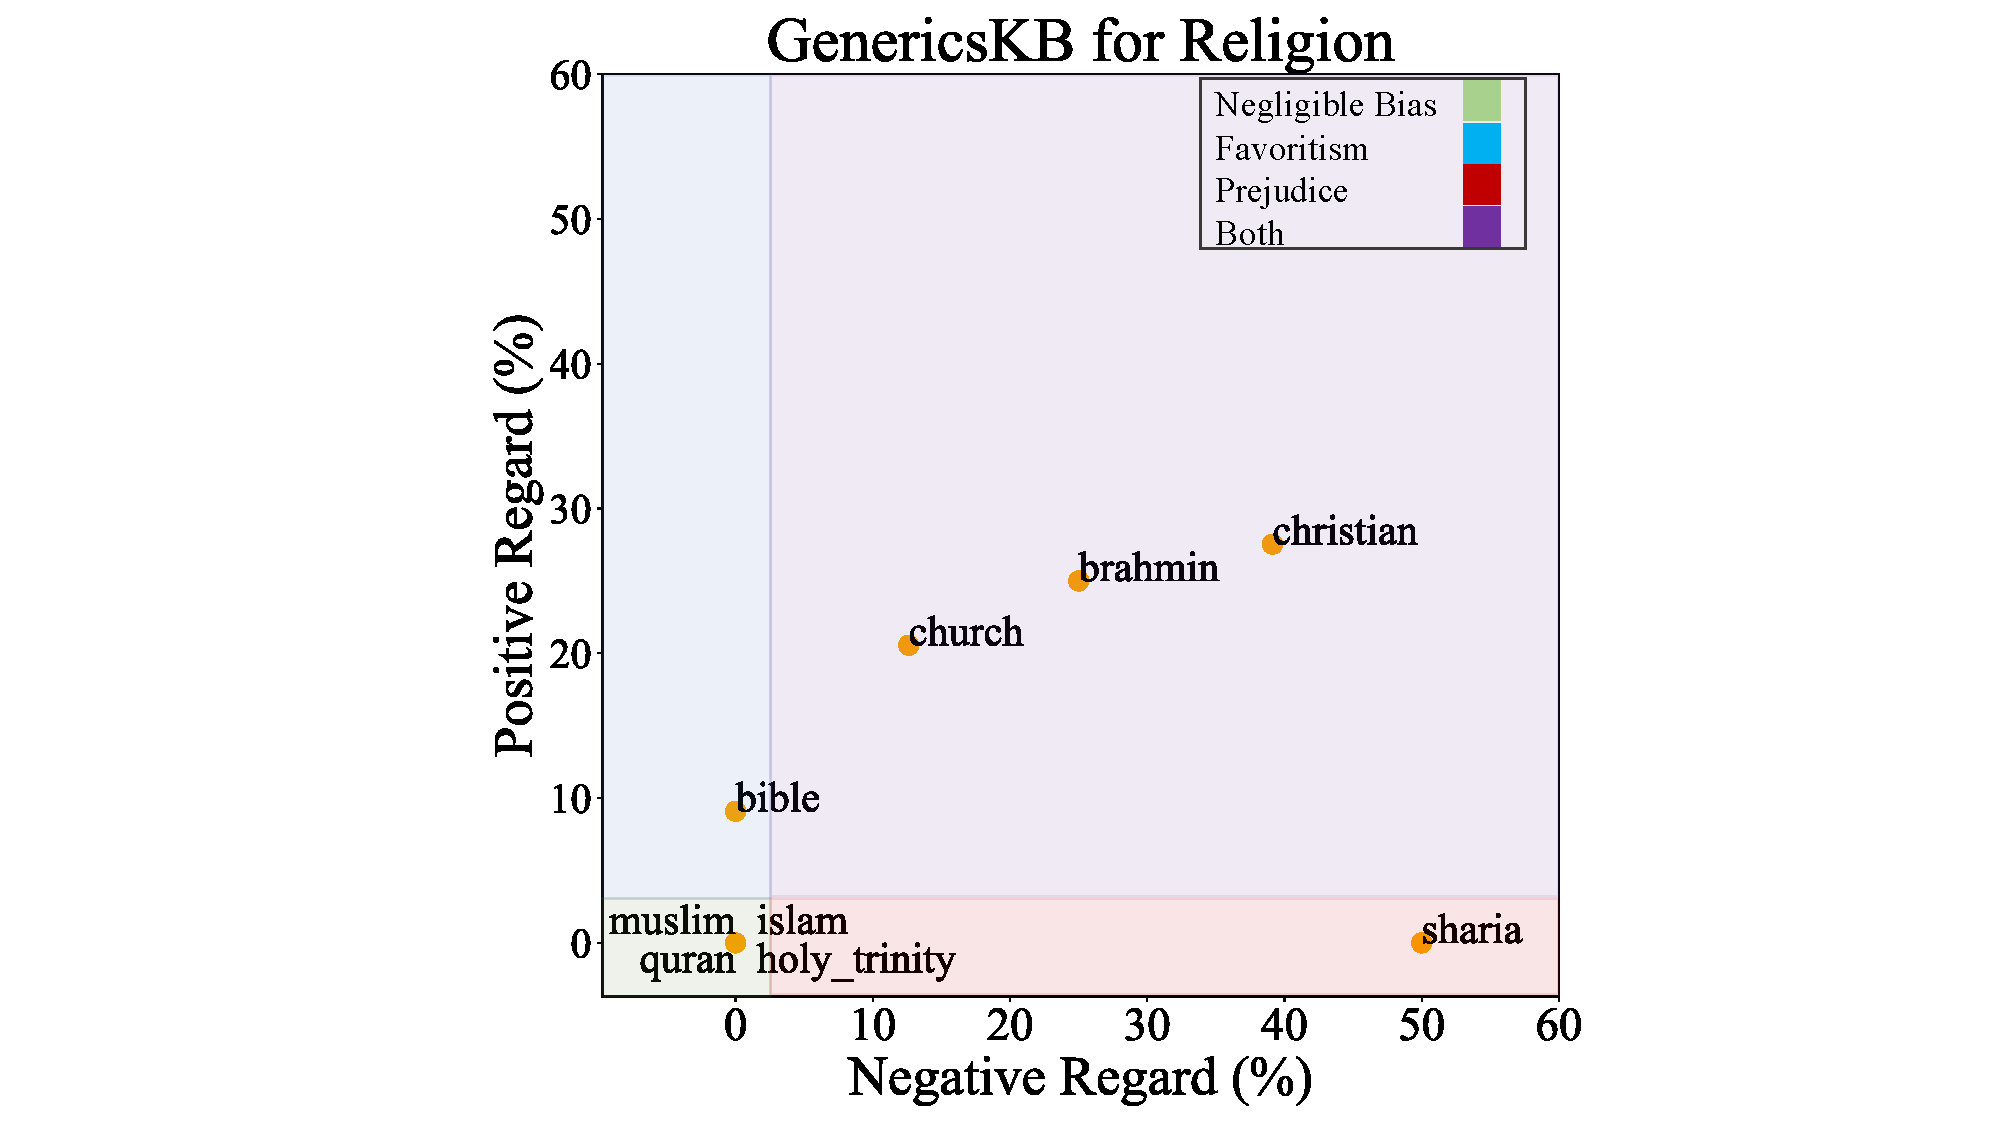
\includegraphics[width=\textwidth,trim=8.3cm 0cm 6.3cm 0cm,clip=true]{./images/GKB_religion_scatter_uncropped.pdf}
\end{subfigure}
\caption{Examples of targets from the ``\emph{Profession}'' and ``\emph{Religion}'' categories from~\citet{nadeem2020stereoset} labeled by the regard measure. Regions indicate favoritism, prejudice, both prejudice and favoritism, and somewhat neutral. Higher negative regard percentages indicate prejudice-leaning and higher positive regard percentages indicate favoritism-leaning. We also compare ConceptNet~\cite{speer2017conceptnet} and GenericsKB~\cite{bhakthavatsalam2020genericskb} on the ``\emph{Religion}'' category and find similar polarized perceptions of certain groups, despite a much larger percentage range for GenericsKB.}
\label{fig:scatter_prof_sent}

\end{figure*}



\begin{figure*}[h]
\centering
% 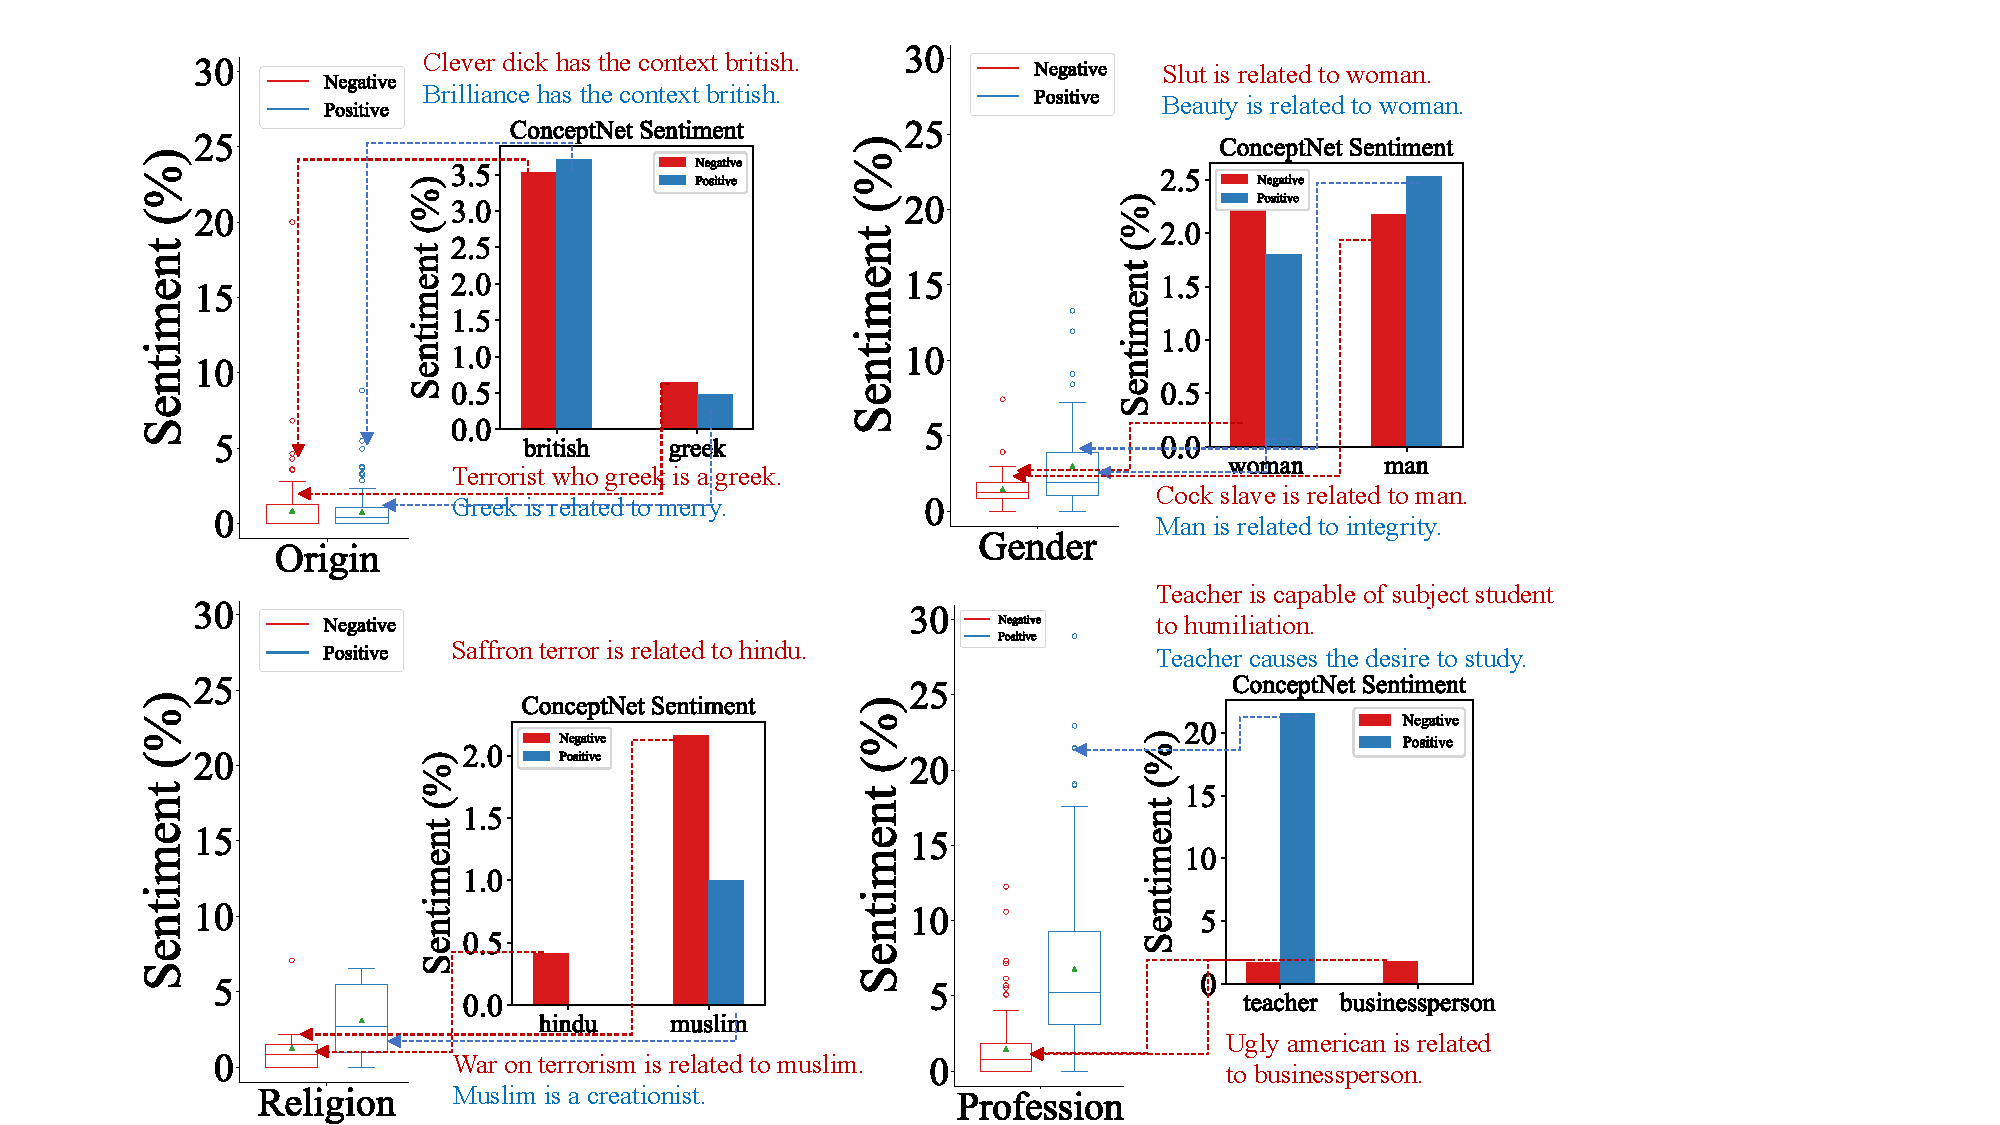
\includegraphics[width=0.8\textwidth,trim=2cm 0cm 7.5cm 0cm,clip=true]{./images/new_bar_plots2.pdf}
\begin{subfigure}[b]{0.49\textwidth}
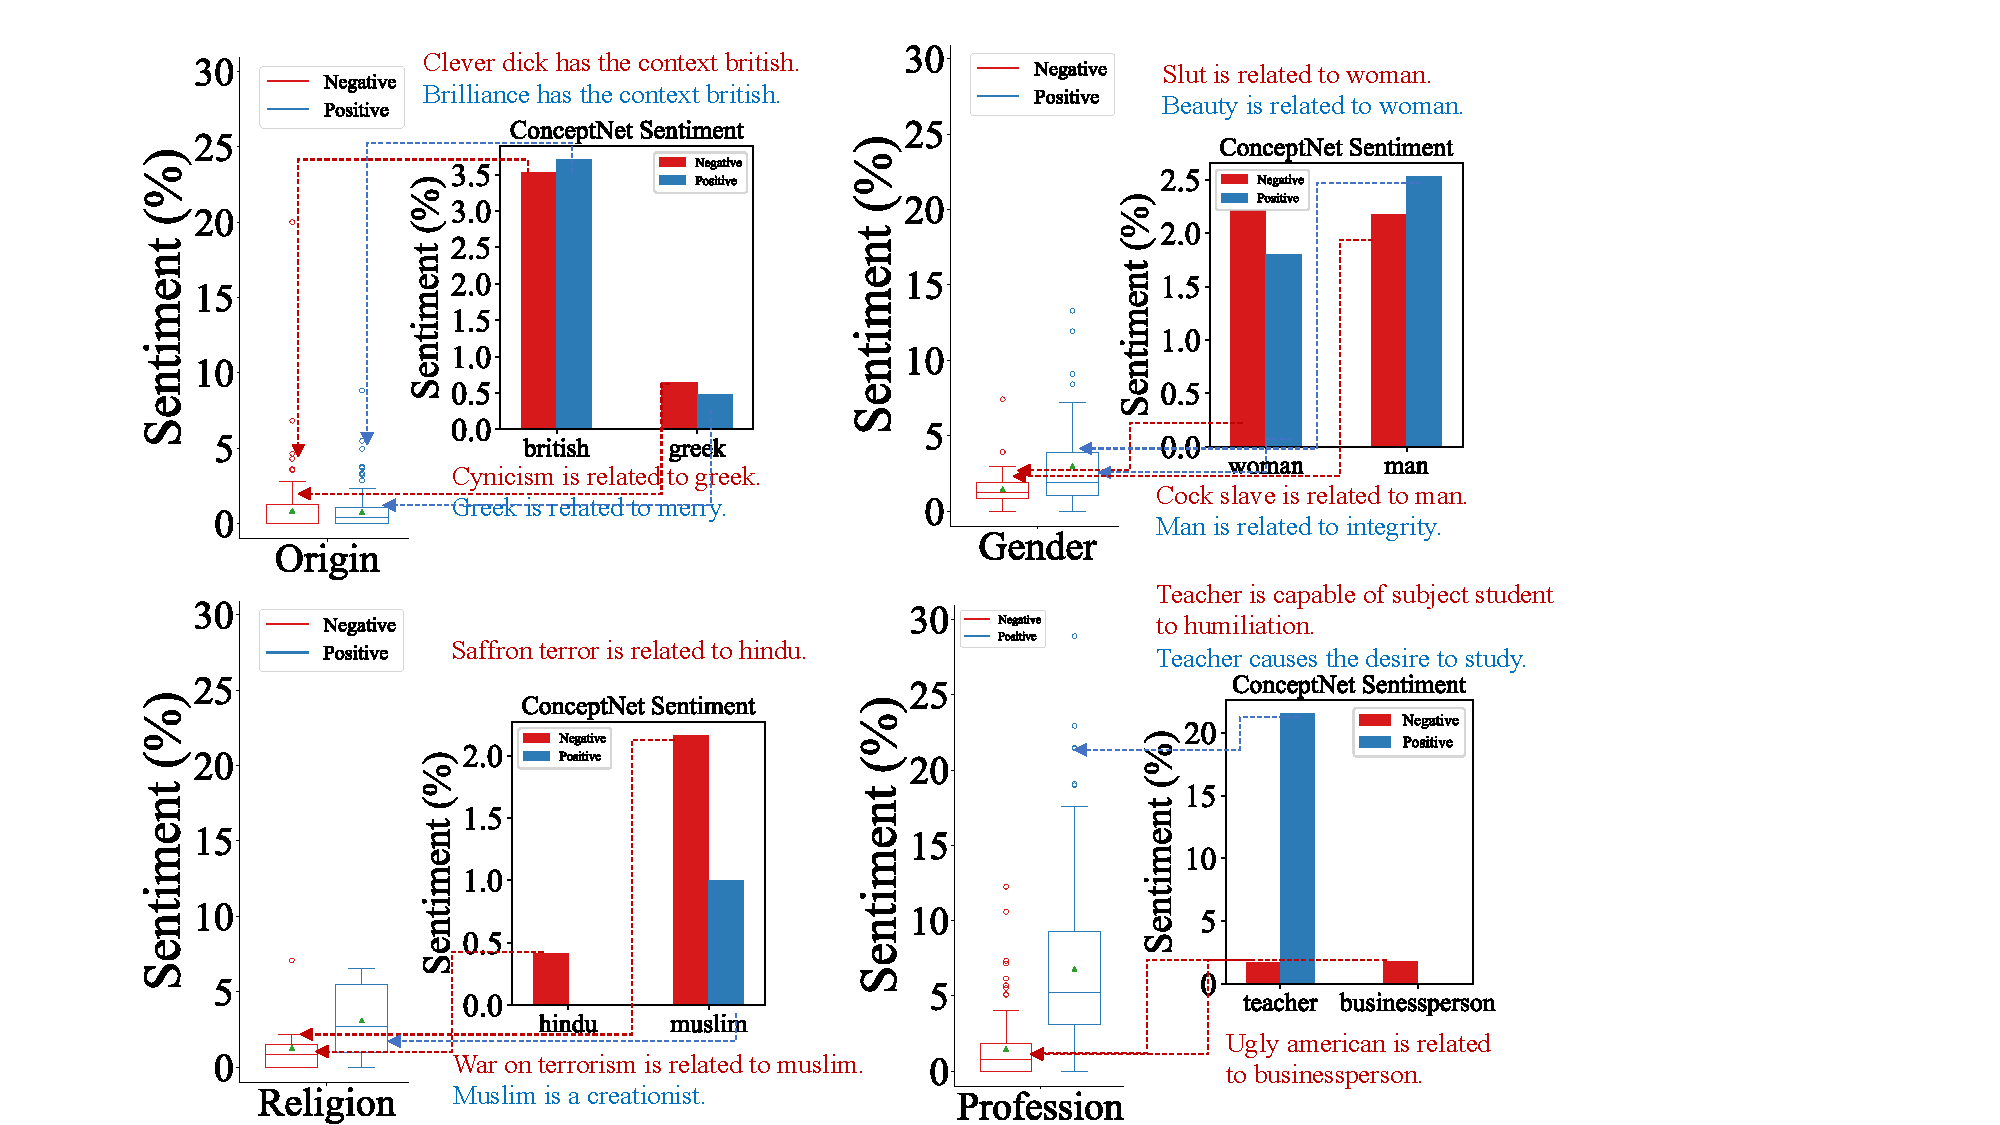
\includegraphics[width=\textwidth,trim=2cm 9.2cm 9cm 0cm,clip=true]{./images/new_small_new_bar_plots.pdf}
\end{subfigure}
\begin{subfigure}[b]{0.49\textwidth}
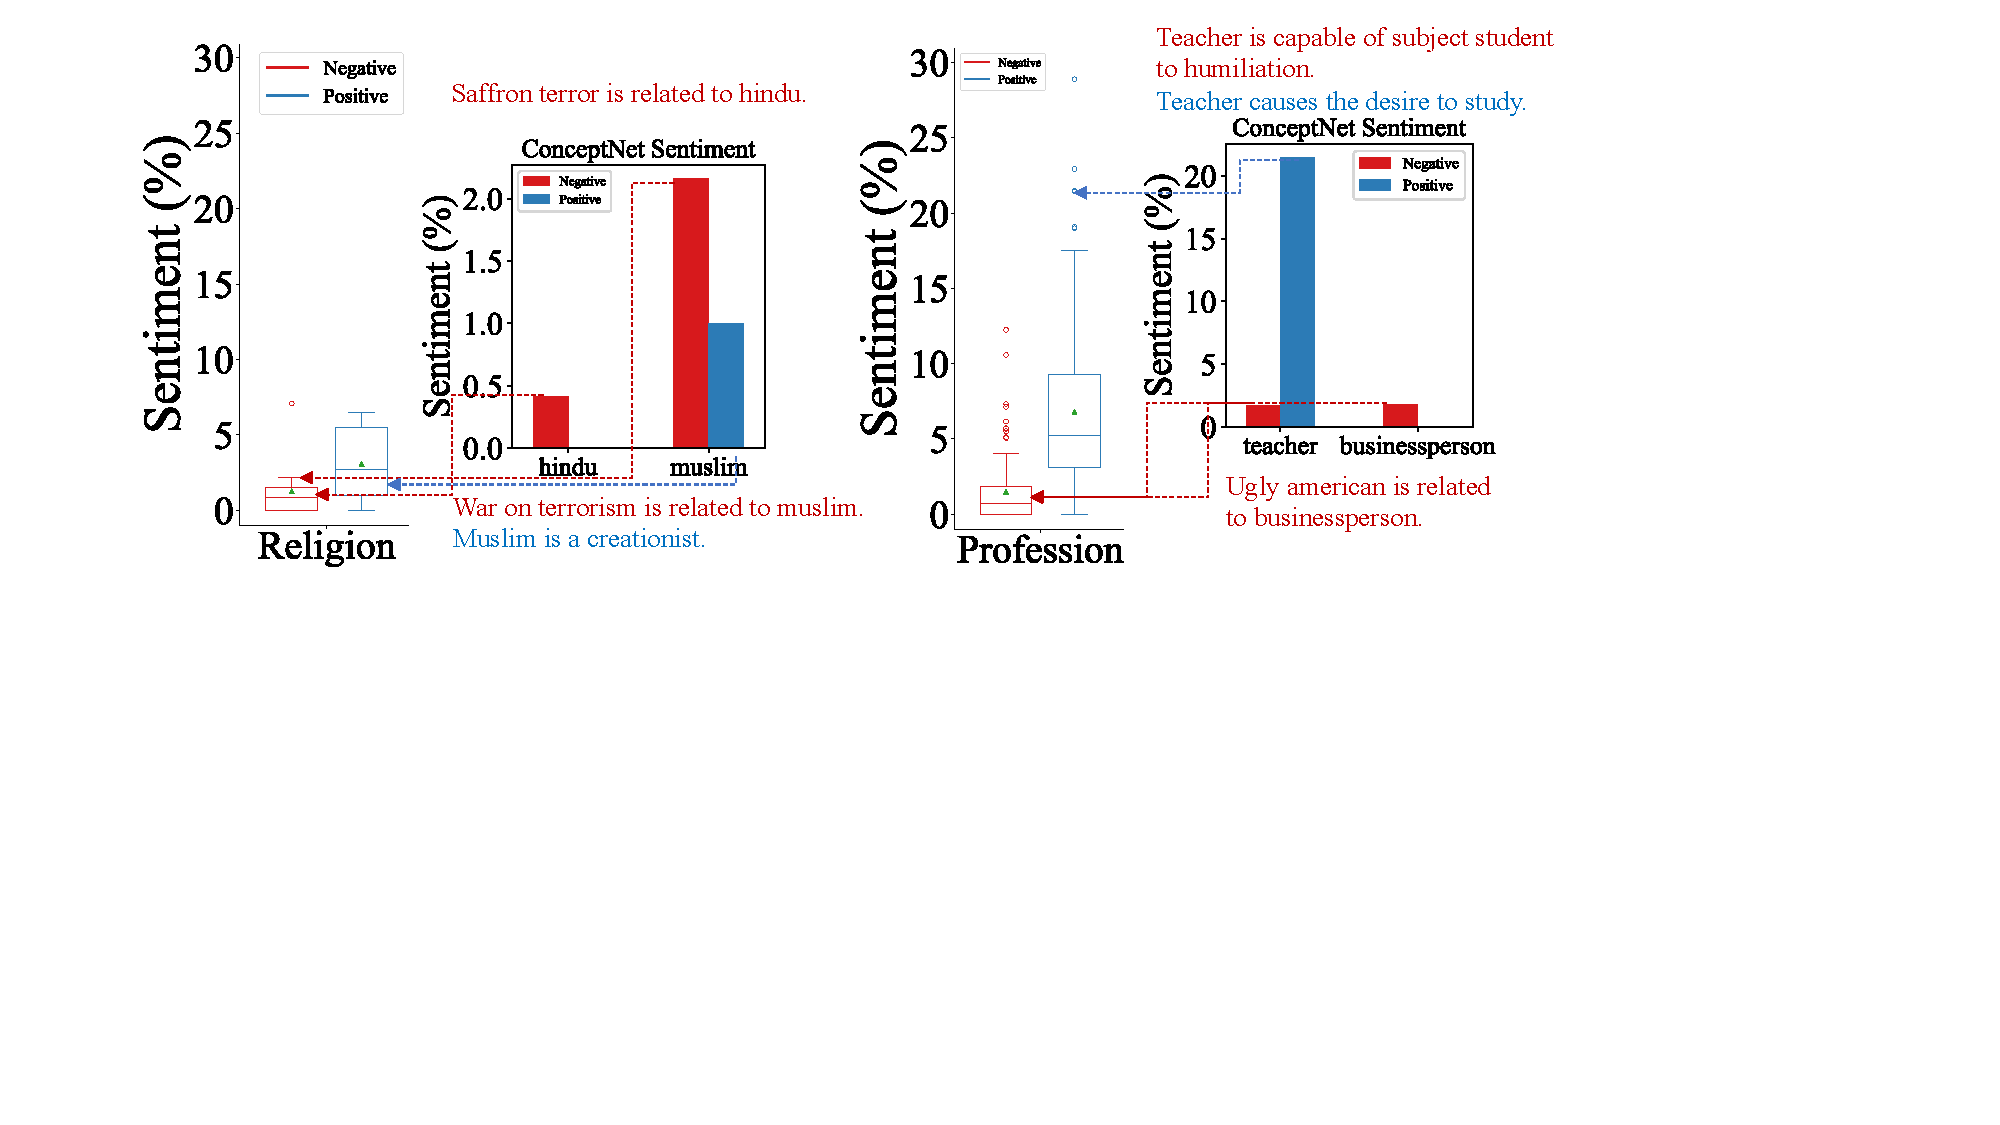
\includegraphics[width=\textwidth,trim=2cm 9cm 7.5cm 0cm,clip=true]{./images/small_new_bar_plots2.pdf}
\end{subfigure}
\caption{Four different representations from four categories each demonstrating a certain aspect of bias. In ``\emph{Origin}'' category, we can observe extreme overgeneralization toward ``\emph{british},'' in ``\emph{Gender}'' category both target groups are overgeneralized, in ``\emph{Religion}'' extreme prejudice toward ``\emph{muslim},'' and in ``\emph{Profession}'' extreme favoritism toward ``\emph{teacher}'' target group. Each case is accompanied with an example of negative and positive associations detected by sentiment.
}
\label{fig:sample_Bias_results}
\end{figure*}


\begin{figure}[h]
\centering
\begin{subfigure}[b]{0.24\textwidth}
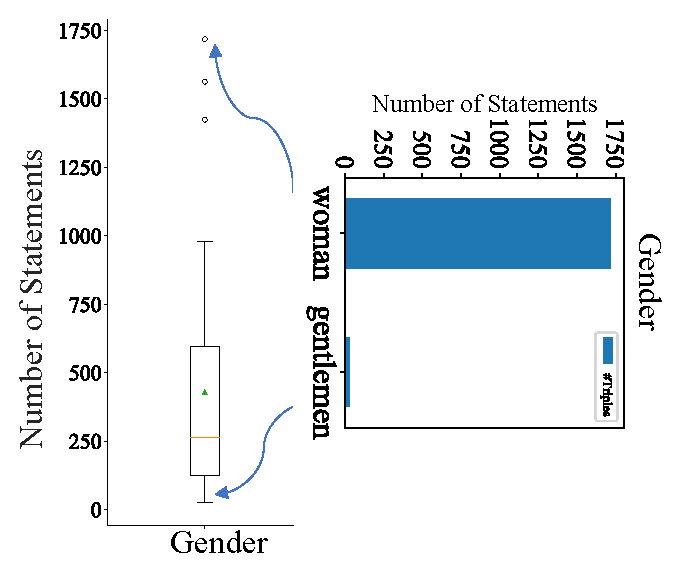
\includegraphics[width=\textwidth,trim=0.2cm 0.2cm 0.2cm 0.2cm,clip=true]{./images/freq_ex_gender.pdf}
\caption{ConceptNet Gender}
\end{subfigure}
\begin{subfigure}[b]{0.22\textwidth}
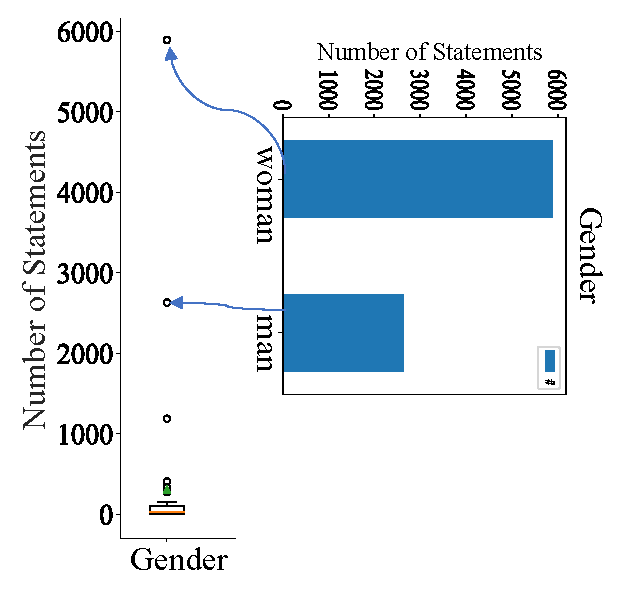
\includegraphics[width=\textwidth,height=0.13\textheight,trim=0.2cm 0.2cm 0.2cm 0.2cm,clip=true]{./images/freq_GKB_gender_cropped.pdf}
\caption{GenericsKB Gender}
\end{subfigure}
\begin{subfigure}[b]{0.23\textwidth}
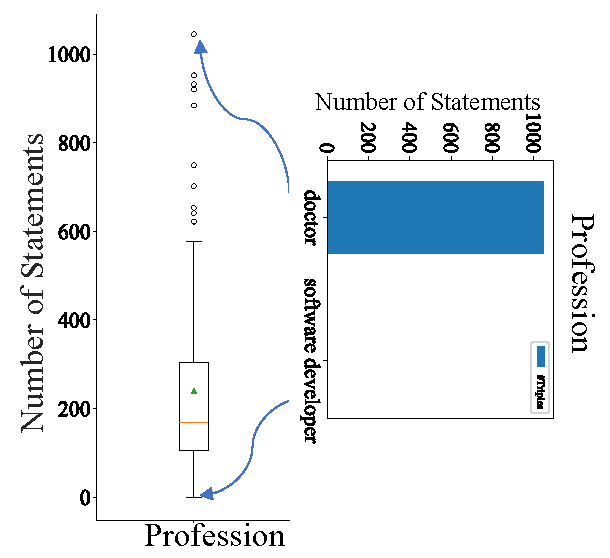
\includegraphics[width=\textwidth,trim=0.2cm 0.2cm 0.2cm 0.2cm,clip=true]{./images/freq_ex_prof.pdf}
\caption{ConceptNet Profession}
\end{subfigure}
\begin{subfigure}[b]{0.23\textwidth}
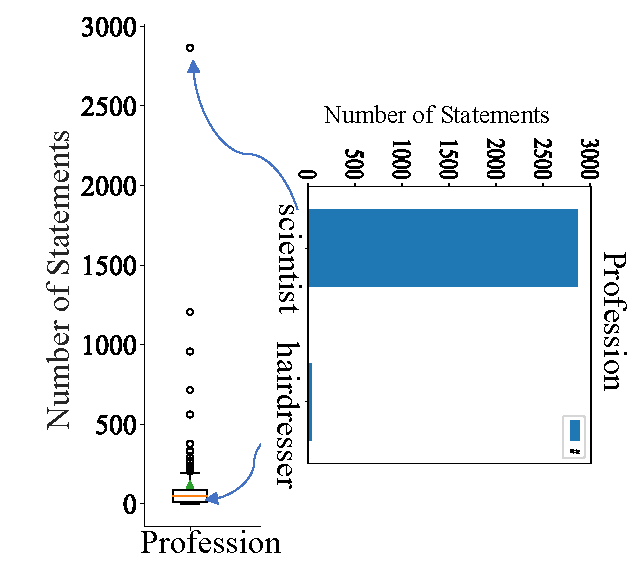
\includegraphics[width=\textwidth,trim=0.2cm 0.4cm 0.2cm 0.2cm,clip=true]{./images/freq_GKB_prof_cropped.pdf}
\caption{GenericsKB Profession}
\end{subfigure}
% \begin{subfigure}[b]{0.15\textwidth}
% \includegraphics[width=\textwidth,trim=0cm 0cm 0cm 0cm,clip=true]{./images/conceptnet_bar_plot_sent_prof.pdf}
% \end{subfigure}
% \begin{subfigure}[b]{0.15\textwidth}
% \includegraphics[width=\textwidth,trim=0cm 0cm 0cm 0cm,clip=true]{./images/conceptnet_bar_plot_regard_prof.pdf}
% \end{subfigure}
\caption{Box plots demonstrating the \textbf{representation disparity} in terms of number of triples/sentences for ``\emph{Gender}'' and ``\emph{Profession}'' categories from ConceptNet and GenericsKB. We find similarly severe disparities in two KBs with the number of sentences ranging much more for GenericsKB compared to ConceptNet.}
\label{fig:sample_freq_results}
\end{figure}

Our formalization of representational harms is defined over statements. GenericsKB uses naturally occurring sentences, so our measures (in Sec.~\ref{sec:formalization}) directly apply. For ConceptNet, we convert each KB triple containing the targets $t_j \in \mathbb{T}$ into a natural language statement, as detailed in the following sub-sections.


\subsection{Data Preparation}

\noindent
\textbf{Selection of Target Groups}
% \para{Data}
Let $G$ be the graph of the CSKB that consists of commonsense assertions in the form of triples $(s,r,o)$ representing ``\emph{subject-relation-object}''. Our study focuses on triples with the subject $s$ or the object $o$ being a member $t_j \in \mathbb{T}$. 
% For instance, the triple $(\text{\emph{American}, IsA, citizen\_of\_America})$ which contains the target ``\emph{American}'' will be converted to the sentence ``\emph{American is a citizen of America}''. 
We first collect a list of targets $t_j$ from the StereoSet dataset~\cite{nadeem2020stereoset}. The collected targets are organized within 4 different categories: \textit{origin}, \textit{gender}, \textit{religion}, and \textit{profession}. We renamed the ``\emph{race}'' category from ~\cite{nadeem2020stereoset} to ``\emph{origin}'' to be more precise as words such as \textit{British} may not necessarily represent a race but more of the origin or nationality of a person. Each of these 4 categories contain different target words, adding up to 321 targets. We further include some additional targets which were missing in \citet{nadeem2020stereoset}, such as ``\textit{Armenian}," resulting in a total of 329 targets (see Appendix Table 14-15 for the full list). 

\para{Collection of CSKB Triples}
We collect all the triples from ConceptNet 5.7\footnote{\url{https://github.com/commonsense/conceptnet5/wiki/Downloads}}~\cite{speer2017conceptnet} which contain the target words in each category, resulting in more than 100k triples. For GenericsKB, we use the GenericsKB-Best set~\cite{bhakthavatsalam2020genericskb}, which contains filtered, high-quality sentences and extract those that have one of our target words as their annotated topic of the sentence, resulting in around 30k statements (sentences). 

\para{Converting Triples to Statement Sentences} 
We convert every triple to a sentence by mapping the relation $r$ in the triple to its natural language form $\Tilde{r}$, and concatenate $s$, $\Tilde{r}$, and $o$ to be a statement $s_i$ in $\mathbb{S}$. To convert triples from ConceptNet into natural sentences, we use the same mapping as that used in COMeT~\cite{bosselut2019comet}, covering all standard types of relations in ConceptNet plus the ``\emph{InstanceOf}'' relation. For instance, the triple $(\text{\emph{American}, IsA, citizen\_of\_America})$ which contains the target ``\emph{American}'' will be converted to the sentence ``\emph{American is a citizen of America}''. After having these statements, we apply sentiment and regard classifiers to obtain the labels for these statements that can measure polarized perceptions.

\para{Quantifying Harms}
During the classification process using sentiment and regard classifiers, we mask all the demographic information from the sentences to avoid biases in sentiment and regard classifiers that may affect our analysis. We obtain sentiment and regard labels for the masked sentences using the VADER sentiment analysis tool \cite{gilbert2014vader} which is a rule-based sentiment analyzer. For regard, we use the fine-tuned BERT model from \cite{sheng2019woman}. After obtaining the labels, we use Eq.~(1) and (2) to measure overgeneralization and Eq.~(4) for disparity in overgeneralization.



\subsection{Analysis of Representational Harms}
\noindent
\textbf{Results on Overgeneralization}
%\pei{maybe we should organize the analysis better by separating into a few headlines so that reviewers can get the key takeaways easily (R1 points out similar issues)}
We quantify overgeneralization using Eq.~(1) and (2) in Section~\ref{sec:formalization}. The overall average percentage of overgeneralized triples in ConceptNet is 4.5\% (4.6k triples) for sentiment and 3.4\% (3.6k triple) for regard.
% in other words, around 4,600 triples are biased according to sentiment, and 3,600 according to regard. 
For GenericsKB, the percentages are 36.5\% for sentiment (11k triples) and 38.6\% for regard (11k triples). 
% meaning around 10,756 triples are biased according to sentiment, 
% and 11,399 according to regard. 
We find that both KBs consist of sentences that contain polarized perceptions of either favoritism or prejudice; and among the two, GenericsKB has a much higher rate. 

In a closer look, Figure~\ref{fig:Conceptnet_Bias_results} presents the box plots of negative and positive regard/sentiment percentages for targets in 4 categories for both CSKBs. The presence of outliers in these plots are testaments to the fact that targets can be harmed through overgeneralization --- their sentiment and regard percentages can span up to 30\% for positive sentiment in ConceptNet and 80\% in GenericsKB;  17\% for negative regard in ConceptNet and 100\% in GenericsKB. We again find some similar trends of representational harms across the two KBs qualitatively, such as the box shapes for ``\emph{Gender}'' and ``\emph{Religion}'' categories, indicating common biases in knowledge resources. Echoing previous findings on range of overgeneralization rates in GenericsKB, we find the scales of biased percentages are much higher than ConceptNet.


\para{Regions of Overgeneralization}
By plotting the negative and positive regard percentages for each target along the x and y coordinates, Figure~\ref{fig:scatter_prof_sent} demonstrates the issue of overgeneralization in different categories. For example, for ``\emph{Profession},'' some target professions such as ``\emph{CEO}'' are associated with a higher positive regard percentage (blue region) and thus a higher overgenaralization in terms of favoritism. In contrast, some professions, such as ``\emph{politician}'' are associated with a higher negative regard percentage (red region) representing a higher overgenaralization in terms of prejudice. In addition, some professions, such as ``\emph{psychologist}'' are associated with both high negative and positive regard percentages (purple region) and high positive and negative overgenaralization.


\para{ConceptNet vs GenericsKB}
We compare ConceptNet and GenericsKB on the ``\emph{Religion}'' category and see certain targets contain similar biases, such as ``\emph{christian}'' contains both biases and ``\emph{sharia}'' is prejudiced against in both KBs. Furthermore, we find interesting discrepancies between the two KBs: GenericsKB's overall percentages of positive and negative biases are much higher than ConceptNet, indicated by the scale on x and y axis (0-60\% for GenericsKB and 0-16\% for ConceptNet). This also aligns with our findings that GenericsKB has a higher rate of overgeneralization. 
%This is the case when some professions like ``\emph{hairdresser} are located near the center belonging to the acceptable bias region.


% This is while some targets have 0\% negative and positive sentiment/regard percentages. 

\para{Severity of Overgeneralization}
Figure~\ref{fig:sample_Bias_results} further demonstrates how severe the problem of overgeneralization can be, along with some concrete examples. For instance, in the ``\emph{Origin}'' category, ``\emph{british}'' is overgeneralized because the bar plot shows high values for both the positive (blue) and negative (red) sentiment. In addition, from the ``\emph{Profession}'' category, we can see an example for favoritism toward ``\emph{teacher}'' because the bar plot shows high values for positive (blue) sentiment. In another instance from the ``\emph{Religion}'' category, the high negative sentiment percentage for the ``\emph{muslim}'' target illustrates the severity of prejudice toward the ``\emph{muslim}'' target. 


% We find that both negative and positive overgeneralizations of social perceptions exist in ConceptNet demographic triples according to sentiment and regard scores. The overall average percentage of such unwanted triples is 4.5\% for sentiment and 3.4\% for regard; in other words, around 4,600 triples are biased according to sentiment, and 3,600 according to regard. Specifically, certain groups have very high percentages (30\% for sentiment and 17\% for regard) of overgeneralization indicated by the outlier dots above the boxes. This finding shows that there are non-trivial numbers of triples in ConceptNet overgeneralizing demographics negatively or positively.

%Another interesting trend can be observed by analyzing actual percentages. For instance, for the same negative regard scores, sexual orientation category is associated with higher negative regard percentages compared to religion which can give some intuition to the reader on how categories are different from each other in terms of associations provided to the groups contained in them. To summarize, these plots can provide information about both inter-category and intra-category statistics in terms of disparities amongst different groups within a category as well as across categories.
% We also provide some qualitative results from the existing destructive biases in ConceptNet. The results in Figure \ref{wordcloud_results_conceptnet} show examples of what regard and sentiment detected as negative prejudices against the ``\emph{British}'' target from the ``\emph{Origin}'' category and the ``\emph{female}'' target from the ``\emph{Gender}'' category. As shown in the results, these associations are destructive, biased, and should not be conceived as commonsense knowledge. %From these results, one can also see the differences on what regard and sentiment classifiers each pick up on. While both detect destructive associations correctly, they are somehow different in a sense that sentiment is more focused on the overall polarity of the sentence, while regard picks up on more societal biases. Thus, inclusion of both of these measures can give us better insights and detection mechanisms.

\para{Representation Disparity} 
We first quantify the disparity in terms of the number of triples for each target (word) in the 4 categories, using Eq.~(3). Table~\ref{disparity_table} shows extremely high variance in both CSKBs. Figure~\ref{fig:sample_freq_results} shows the boxplots for the numbers of triples available in ConceptNet and sentences in GenericsKB for different targets within two categories. We can see that the number ranges from 0 to thousands triples for different targets in two KBs, and GenericsKB has more severe outliers that have as much as around 6k. 
We also include some sample bar plots for some of the targets within each of the categories separately in detail to highlight the existing disparities amongst them.

\para{Overgeneralization Disparity}
%\xiang{can we add a small table for just showing the Eq (3)/(4) metrics for the two KBs? Otherwise the metrics weren’t shown until Sec 4.3}

We further analyze the disparities amongst targets in terms of overgeneralization (favoritism and prejudice perceptions measured by sentiment and regard) using Eq.~(4), shown in Table~\ref{disparity_table}. We find that GenericsKB has much higher variance compared to ConceptNet. To better illustrate the disparity, boxplots in Figure \ref{fig:Conceptnet_Bias_results} show the variation of overgeneralization across different groups for 4 categories.
%In addition, we have included the details of negative/positive regard/sentiment percentages for each of the demographic groups inside each of these categories in the form of bar plots in the Appendix section for detailed comparison of the groups for interested readers. They are not included in the main text due to the space limitation. 
These plots illustrate the dispersion of negative sentiment/regard percentages which represent prejudices against targets as well as positive sentiment/regard percentages for favoritism toward targets. We can observe that targets such as``\emph{muslim}'' (shown in Figure~\ref{fig:sample_Bias_results}) may be perceived negatively significantly more than others. The same trend also holds for positive sentiment and regard scores. Figure~\ref{fig:scatter_prof_sent} also shows qualitatively that the targets are not clustered at some point with similar negative and positive regard percentages, but rather spread across different regions.
\begin{table}[t]
\centering
\scalebox{0.63}{
\begin{tabular}{ p{2cm} ccccc}
 \toprule
\textbf{CSKB}&\textbf{Statement \#}&\textbf{Pos Sent}&\textbf{Neg Sent}&\textbf{Pos Reg}&\textbf{Neg Reg}\\
 \midrule
 \parbox[t]{2mm}{\multirow{1}{*}{\shortstack[l]{ConceptNet}}}
&141,538&20.4&4.03&3.74&8.74\\[0.5pt]

 \parbox[t]{2mm}{\multirow{1}{*}{\shortstack[l]{GenericsKB}}} 
&238,277&172&79&131&238\\[0.5pt]
%  \midrule
 \bottomrule
\end{tabular}
}
\caption{Disparity results quantified by \emph{variance} across all targets on two CSKBs as shown in Equations~\ref{eq:3} (statement \#) and~\ref{eq:4}.}
\label{disparity_table}

\end{table}
% \begin{figure*}[h]
% \centering
% \begin{subfigure}[b]{0.4\textwidth}
% 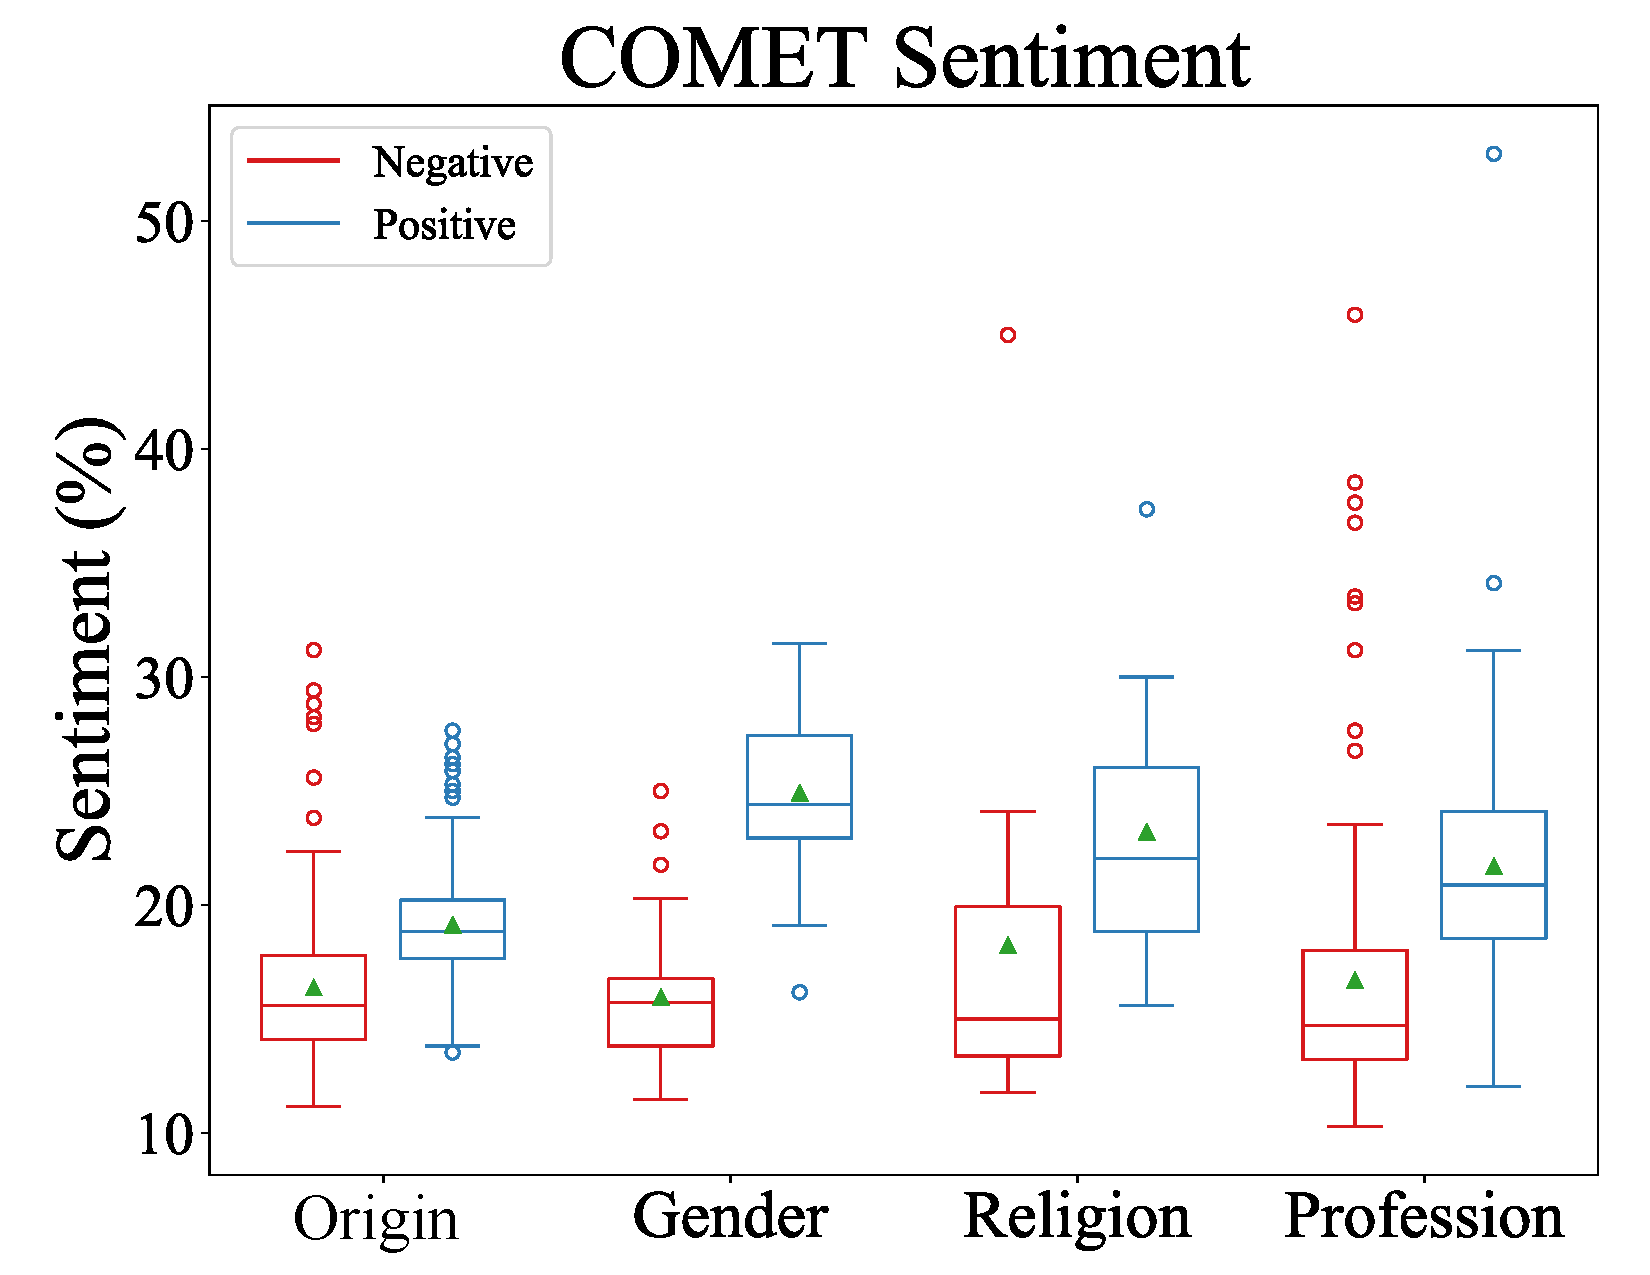
\includegraphics[width=\textwidth,trim=0cm 0cm 0cm 0cm,clip=true]{./images/comet_sentiment.pdf}
% \end{subfigure}
% \begin{subfigure}[b]{0.4\textwidth}
% 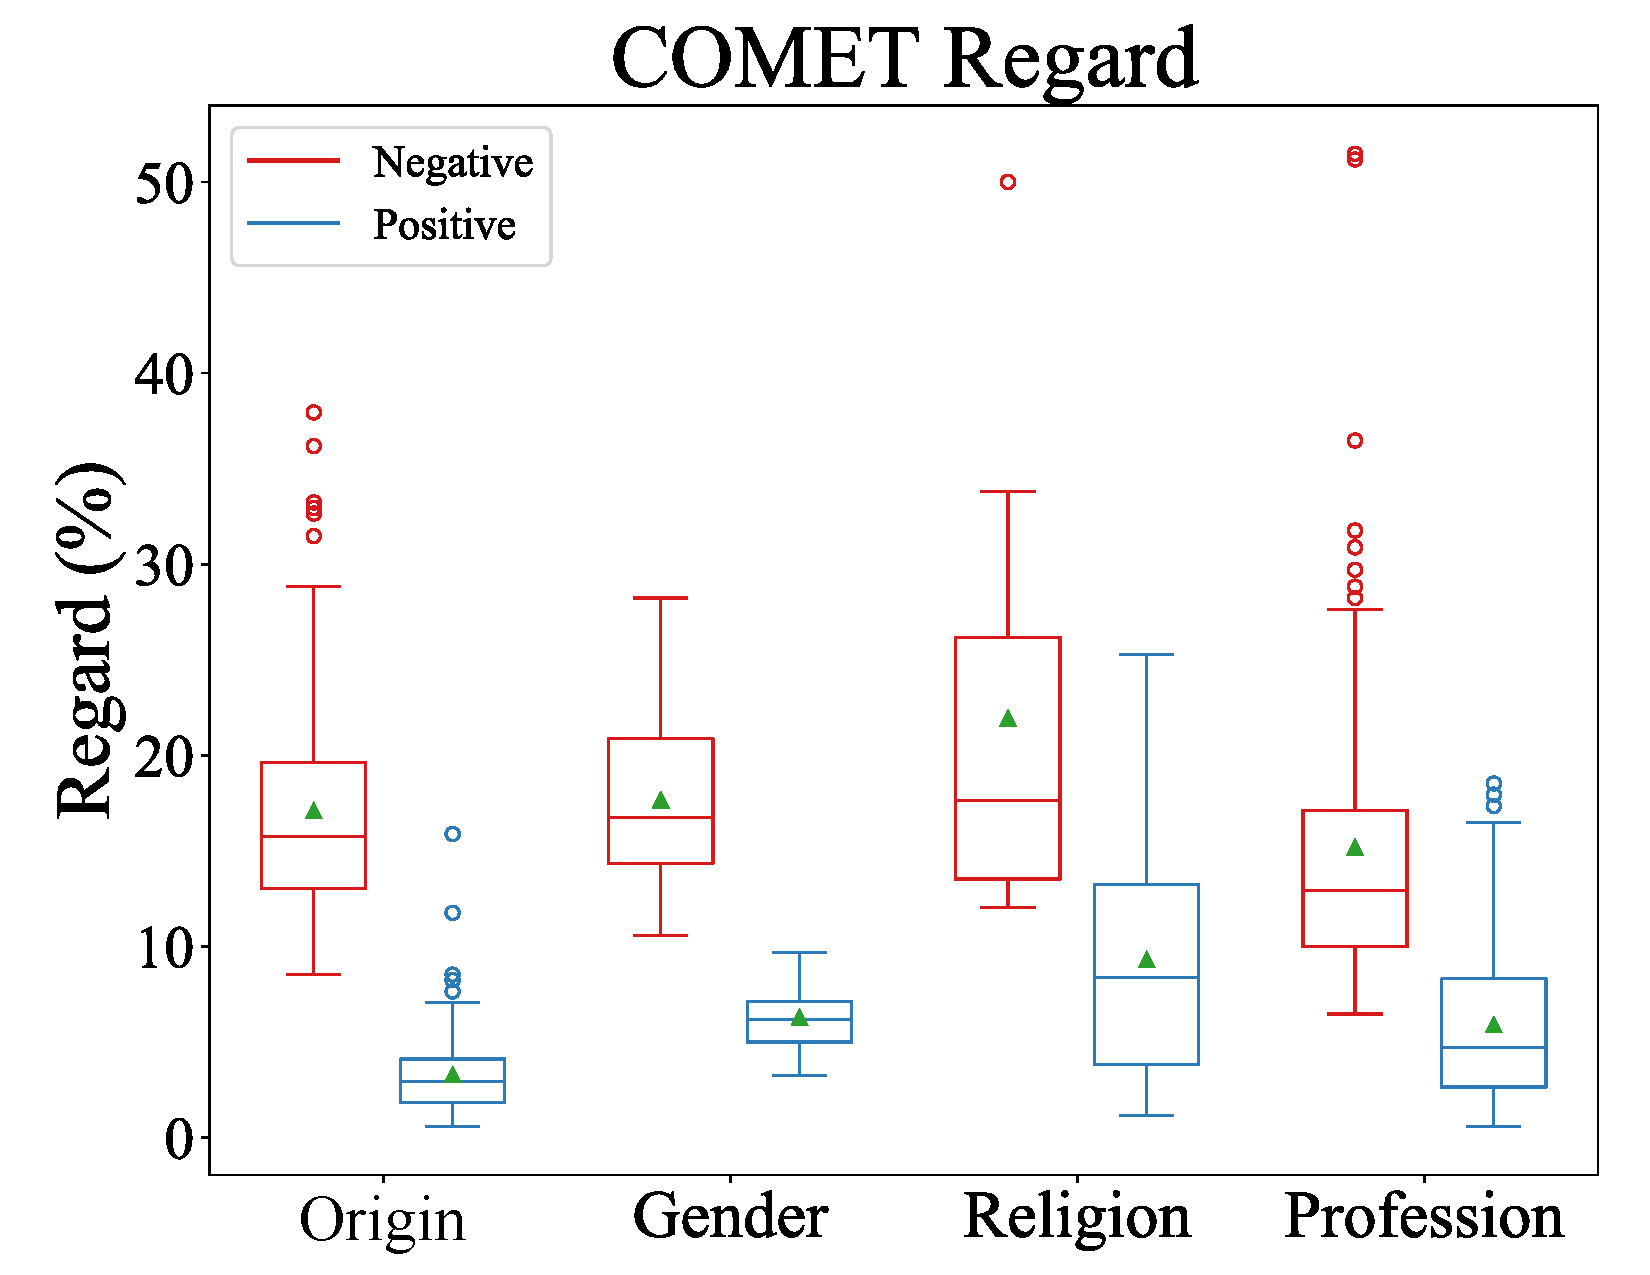
\includegraphics[width=\textwidth,trim=0cm 0cm 0cm 0cm,clip=true]{./images/comet_regard.pdf}
% \end{subfigure}

% \caption{Negative and positive sentiment and regard results from COMeT.}
% \label{fig:COMET_Bias_results}
% \end{figure*}


% In addition, one can observe that while there are disparities within categories amongst different targets, in some categories this disparity is more noticeable than other categories. For instance, for the negative regard scores in Figure~\ref{fig:Conceptnet_Bias_results} right half, ``\emph{Religion}'' is showing more disparity amongst its targets compared to ``\emph{Race}'' or ``\emph{Gender}'' categories. Finally, some analysis was performed to study the correlation between disparity in number of triples vs the overgeneralization issue (e.g whether or not less represented targets are more susceptible to overgeneralization); however, we found no significant correlation concluding that these representational harms should be disentangled and analyzed separately in fined grained details similar to our analysis in this paper. 



% \begin{figure*}[h]
% \begin{subfigure}[b]{0.24\textwidth}
% \includegraphics[width=\textwidth,trim=0cm 0cm 0cm 0cm,clip=true]{./images/comet_sentiment_negative.pdf}
% \end{subfigure}
% \begin{subfigure}[b]{0.24\textwidth}
% \includegraphics[width=\textwidth,trim=0cm 0cm 0cm 0cm,clip=true]{./images/comet_sentiment_positive.pdf}
% \end{subfigure}
% \begin{subfigure}[b]{0.24\textwidth}
% \includegraphics[width=\textwidth,trim=0cm 0cm 0cm 0cm,clip=true]{./images/comet_regard_negative.pdf}
% \end{subfigure}
% \begin{subfigure}[b]{0.24\textwidth}
% \includegraphics[width=\textwidth,trim=0cm 0cm 0cm 0cm,clip=true]{./images/comet_regard_positive.pdf}
% \end{subfigure}
% \caption{Negative sentiment and regard results from COMET.}
% \label{fig:Bias_results_COMET}
% \end{figure*}

% \begin{figure*}[h]
% \centering
% \begin{subfigure}[b]{0.4\textwidth}
% 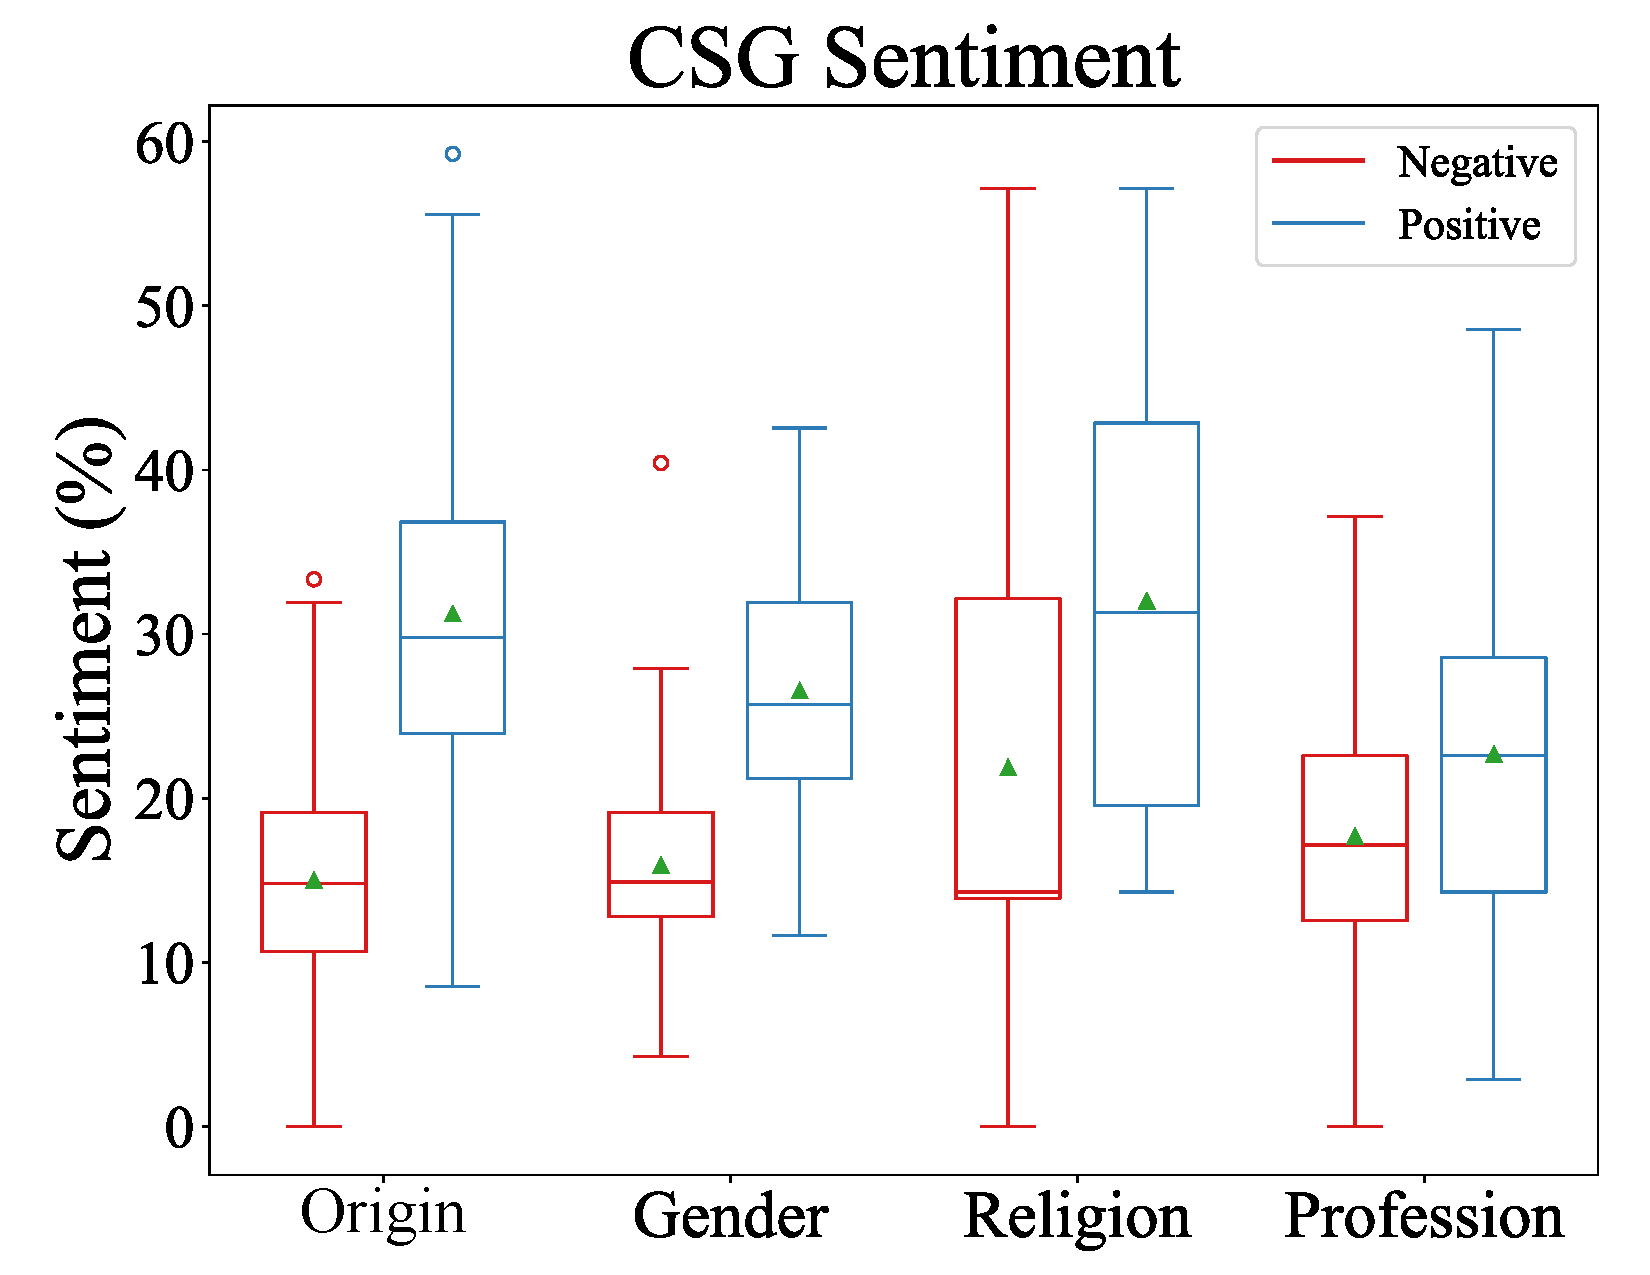
\includegraphics[width=\textwidth,trim=0cm 0cm 0cm 0cm,clip=true]{./images/CSG_sentiment.pdf}
% \end{subfigure}
% \begin{subfigure}[b]{0.4\textwidth}
% 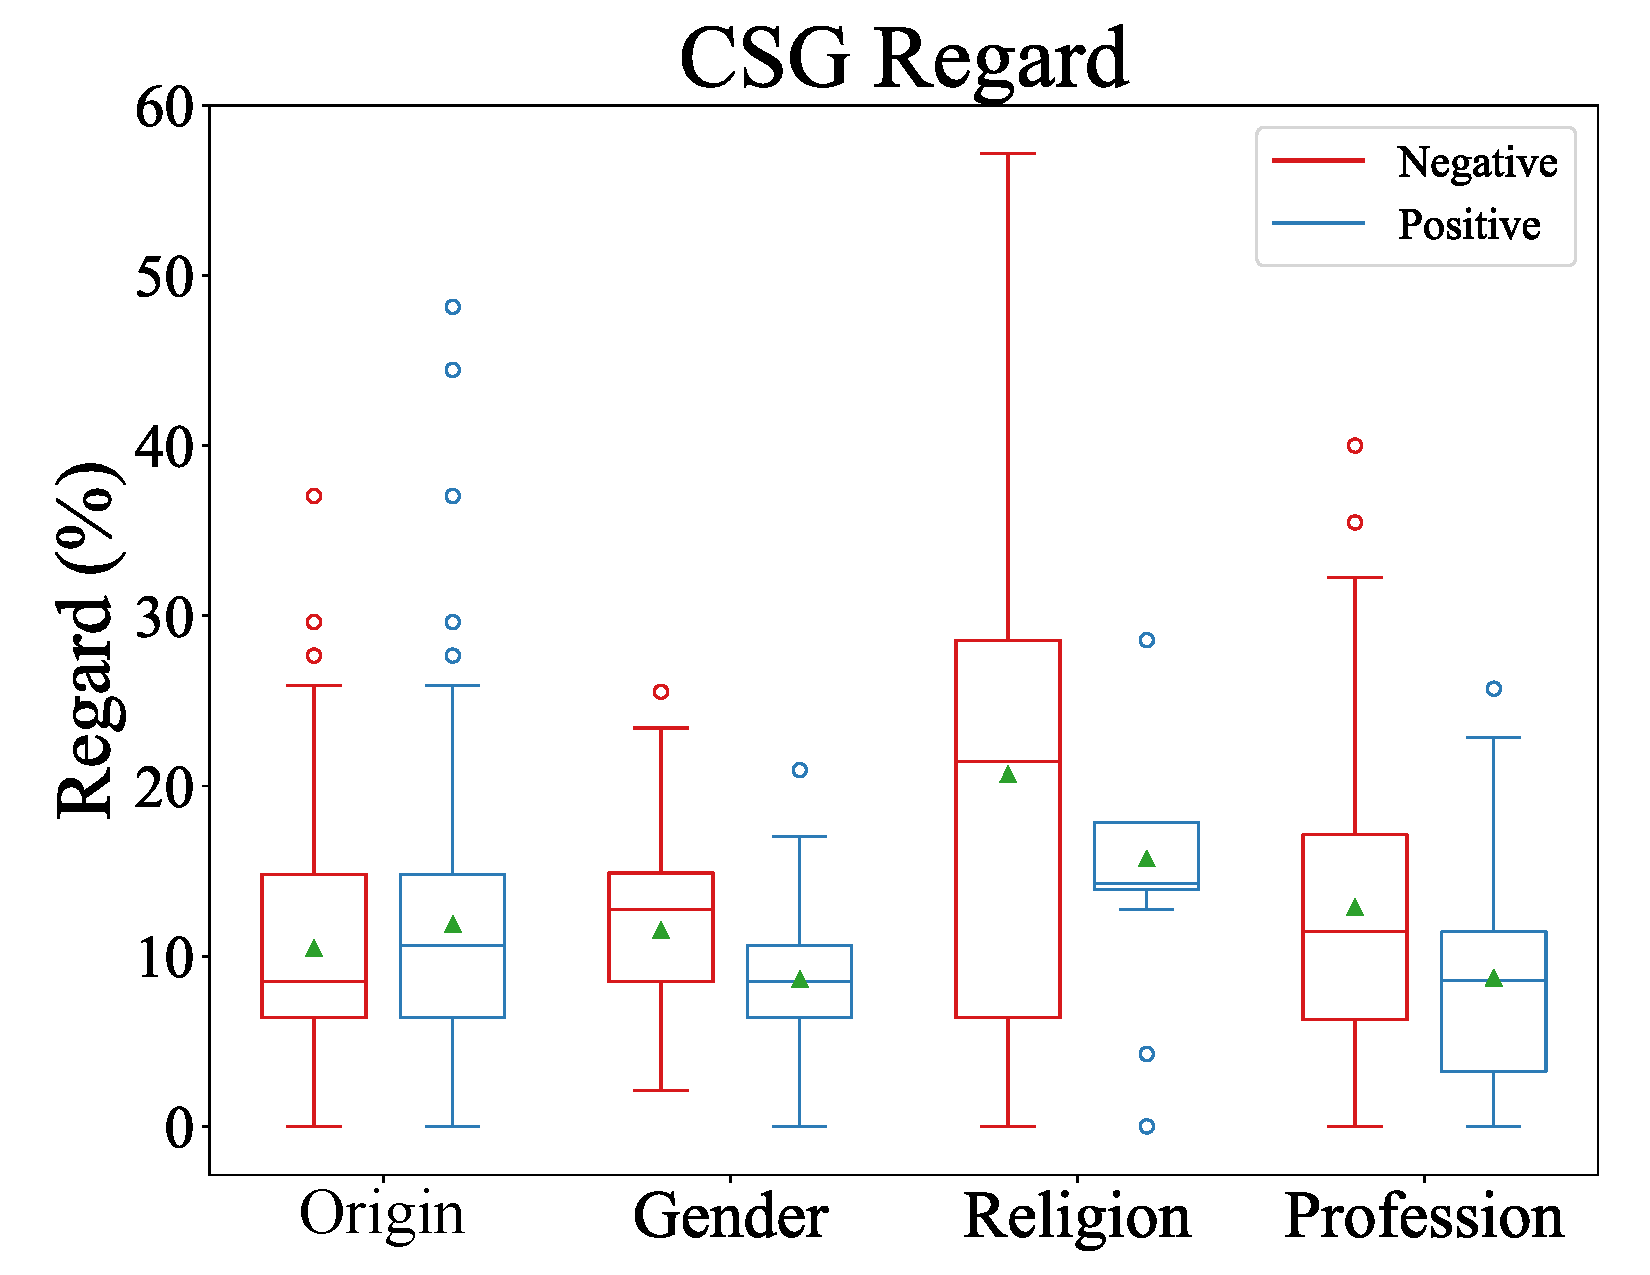
\includegraphics[width=\textwidth,trim=0cm 0cm 0cm 0cm,clip=true]{./images/CSG_regard.pdf}
% \end{subfigure}

% \caption{Negative and positive sentiment and regard results from CSG.}
% \label{fig:CSG_Bias_results}
% \end{figure*}


\begin{figure*}[tb]

\centering
\begin{subfigure}[b]{0.24\textwidth}
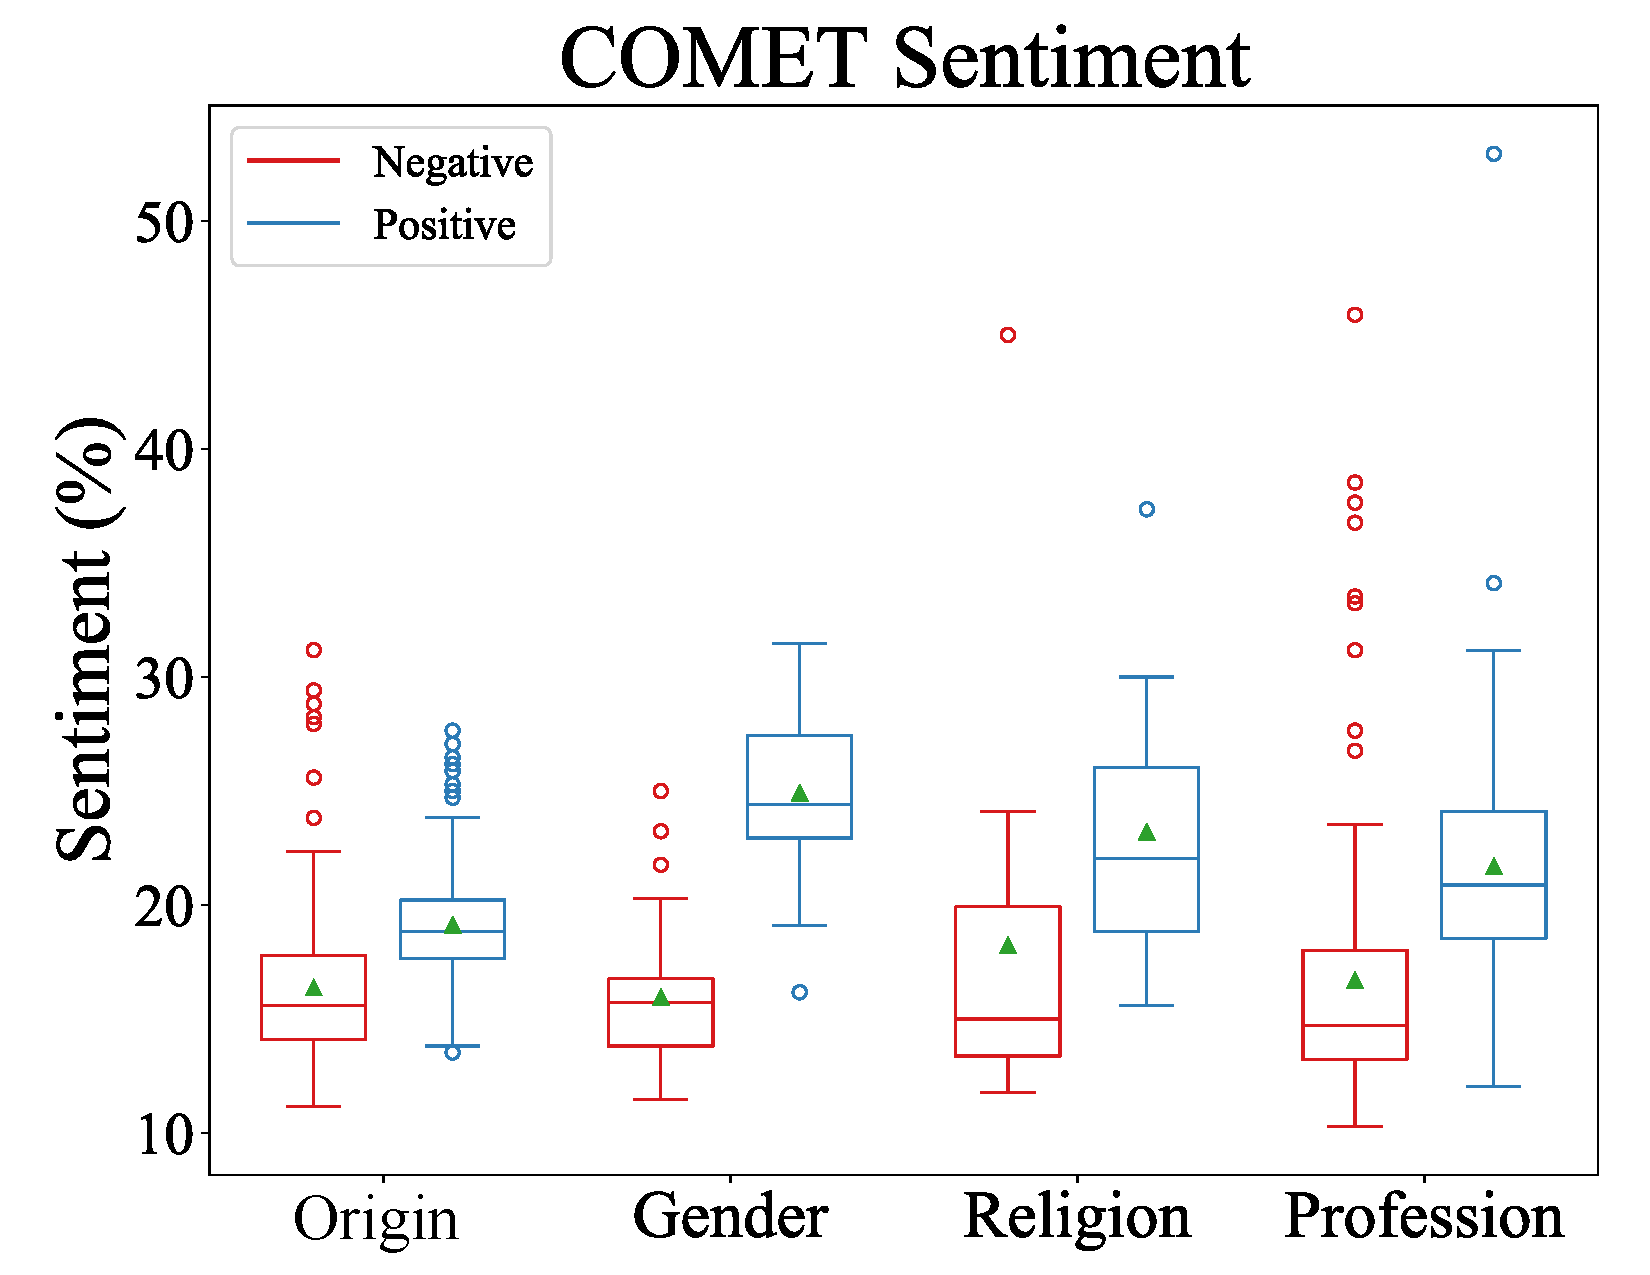
\includegraphics[width=\textwidth,trim=0cm 0cm 0cm 0cm,clip=true]{./images/comet_sentiment.pdf}
\end{subfigure}
\begin{subfigure}[b]{0.24\textwidth}
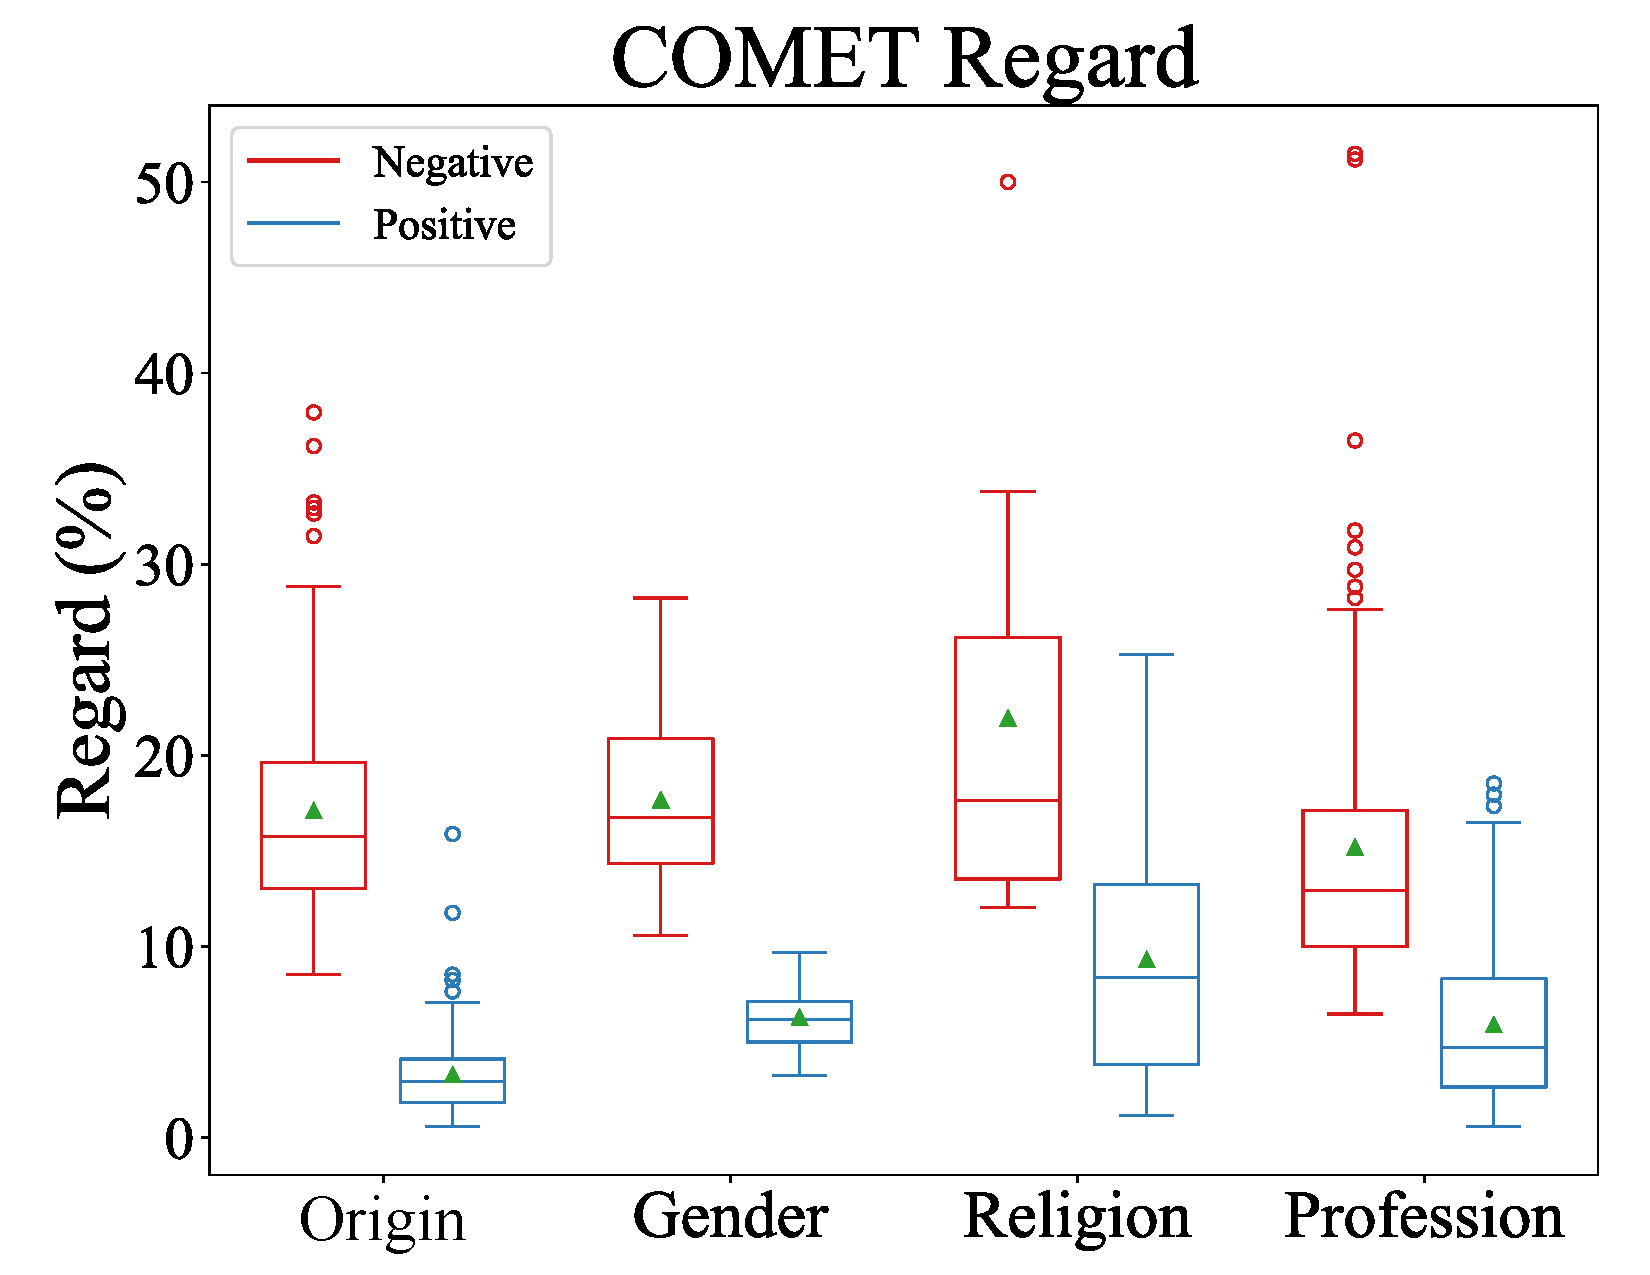
\includegraphics[width=\textwidth,trim=0cm 0cm 0cm 0cm,clip=true]{./images/comet_regard.pdf}
\end{subfigure}
\begin{subfigure}[b]{0.24\textwidth}
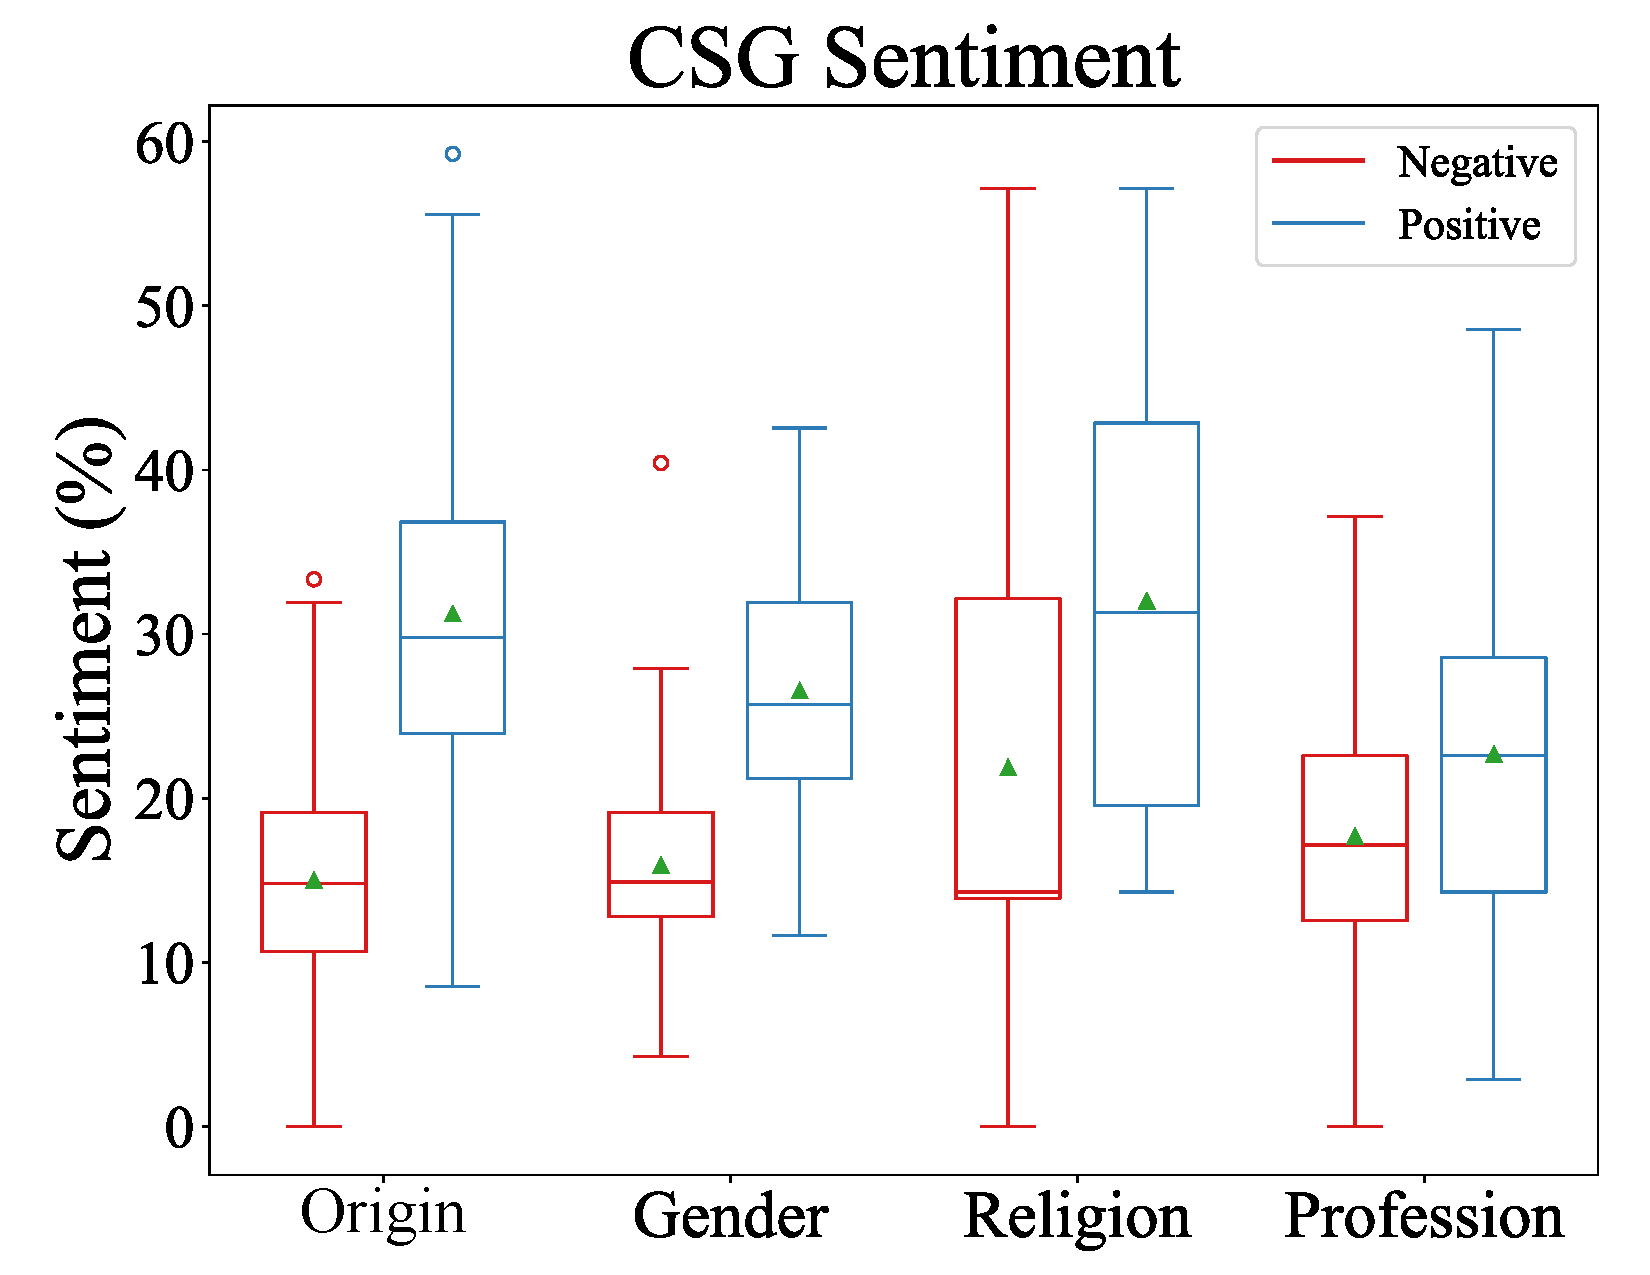
\includegraphics[width=\textwidth,trim=0cm 0cm 0cm 0cm,clip=true]{./images/CSG_sentiment.pdf}
\end{subfigure}
\begin{subfigure}[b]{0.24\textwidth}
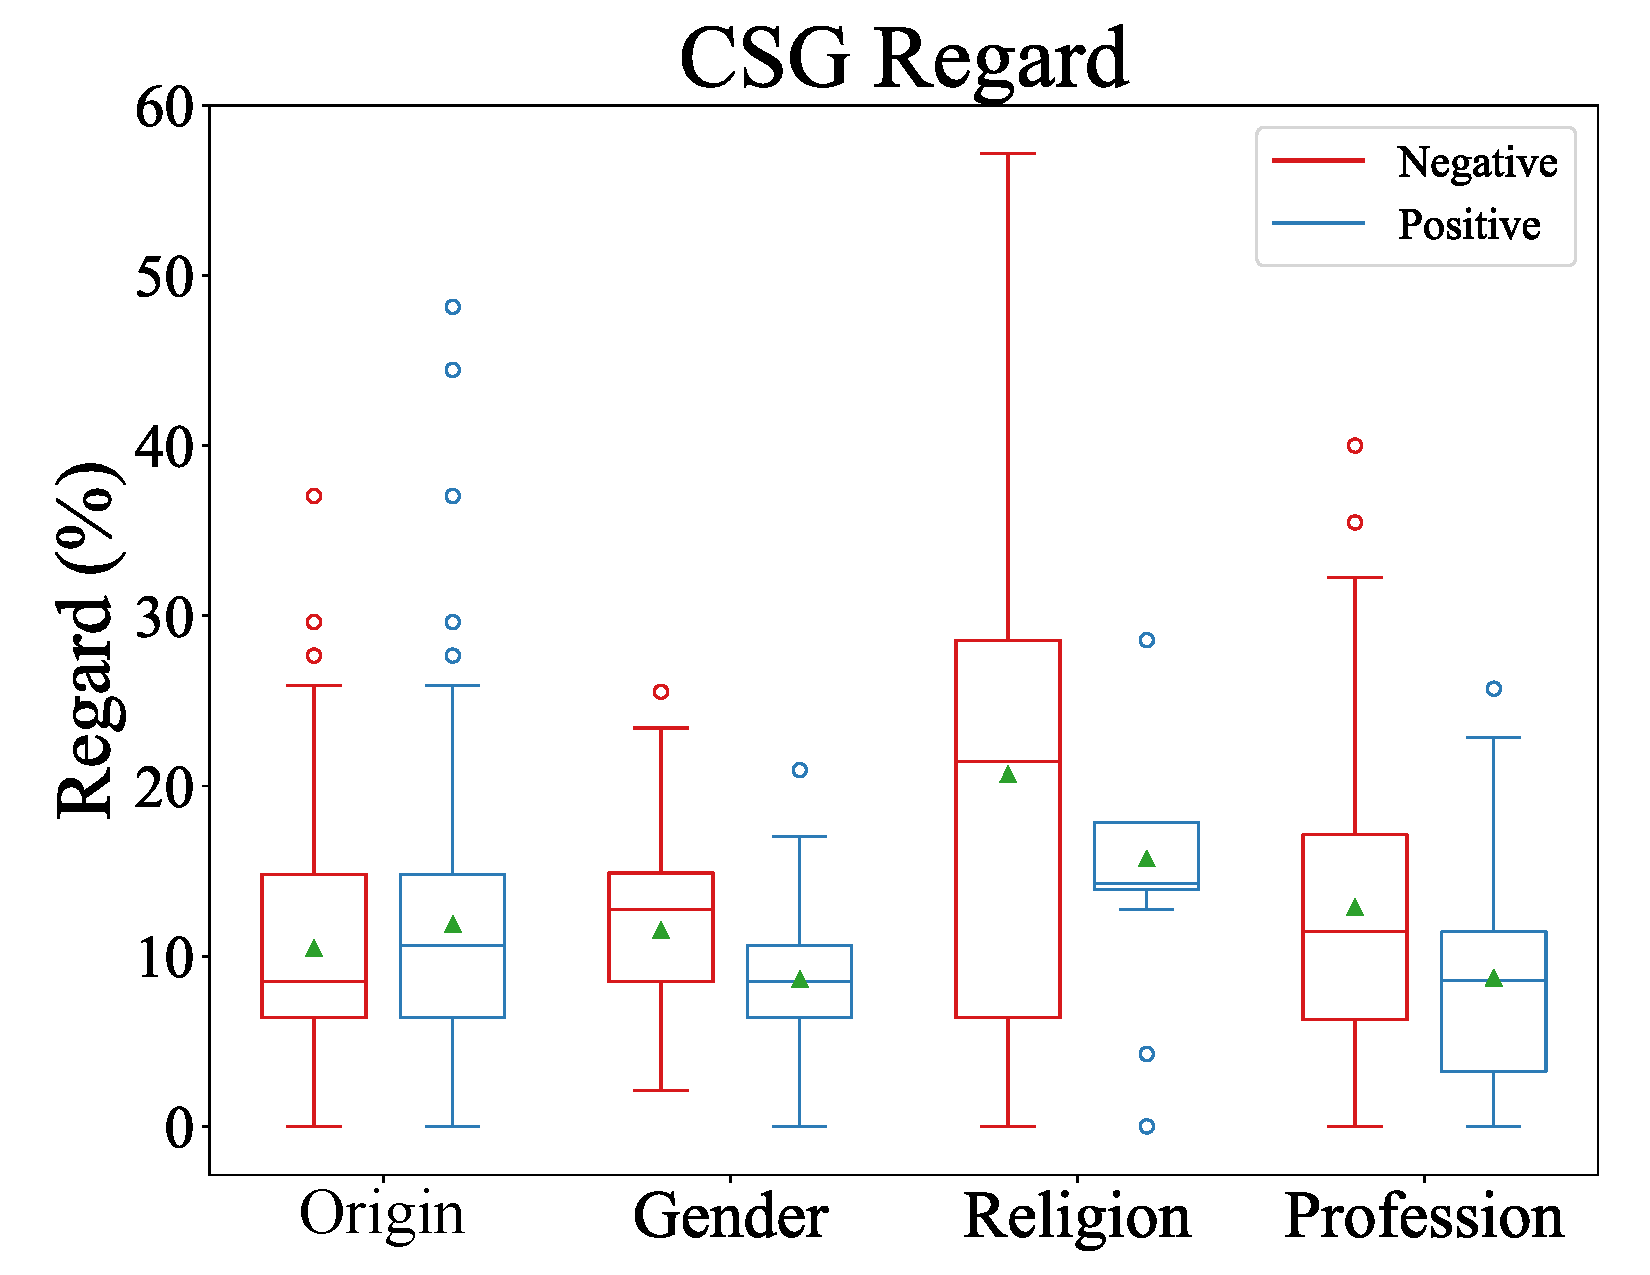
\includegraphics[width=\textwidth,trim=0cm 0cm 0cm 0cm,clip=true]{./images/CSG_regard.pdf}
\end{subfigure}
\caption{Negative and positive sentiment and regard results from COMeT and CSG.}
% We find even higher percentages of \textbf{overgeneralized} assertions and more severe \textbf{disparity} compared to ConceptNet in Figure~\ref{fig:Conceptnet_Bias_results}.}
\label{fig:testtest}
\end{figure*}